% "openany" kell, különben minden fejezet páros lapon kezdődik.
\documentclass[openany]{book}

\usepackage[magyar]{babel}
\defineshorthand{"~}{\babelhyphen{nobreak}}
\useshorthands{"}

\usepackage{fontspec}
\setmainfont{EB Garamond}
\newfontfamily\FateCoreGlyphs[Mapping=tex-text]{Fate Core Glyphs} % dobókocka, cselekvés ikonok
\newfontfamily\Wingdings[Mapping=tex-text]{Wingdings3} % siker/kudarc ikonok
\newfontfamily\Roboto[Mapping=tex-text]{Roboto Light} % példák (Gotham Condensed helyett)
\newfontfamily\RobotoMedium[Mapping=tex-text]{Roboto Medium} % táblázatok (Gotham Condensed helyett)
\newfontfamily\RobotoCondensed[Mapping=tex-text]{Roboto Condensed Bold} % címek (Gotham Condensed helyett)

\usepackage{geometry}
\geometry{a4paper, outer=20mm, inner=30mm, top=20mm, bottom=20mm}

\usepackage{hyperref}
\hypersetup{
    colorlinks=true,
    linkcolor=black,
    urlcolor=gray,
}

\usepackage{titletoc}
\contentsmargin{0pt}
\titlecontents{chapter}[0pt]
     {\RobotoCondensed\Large\bfseries}{}{}{\titlerule*[0.7pc]{.}\thecontentspage}
\titlecontents{section}[0.5em]
     {}{}{}{\titlerule*[0.7pc]{.}\thecontentspage}
\titlecontents*{subsection}[1em]
     {\filright\small}{}{}{}[;\quad]
\setcounter{tocdepth}{2}

\usepackage{titlesec}
\usepackage{graphicx}
\usepackage[table]{xcolor}
\usepackage{multicol}
\usepackage{amsmath}
\usepackage{lettrine}
\usepackage[toc]{multitoc}
\usepackage{wrapfig}

\usepackage{fancyhdr}
\fancyhf{}
% Ez kikapcsolja a default vonalat a header alatt.
\renewcommand{\headrulewidth}{0pt}
\fancyhead[LE]{\textbf{\thepage\quad Fate Condensed \quad\leftmark}}
\fancyhead[RO]{\textbf{Fate Condensed \quad\leftmark \quad\thepage}}
% Ez kell, különben a \chapter oldalakon (ami fixen plain-t használ) nem lesz header, csak oldalszám footer.
\fancypagestyle{plain}{}

% Ez a szürke csík a \example oldalán.
\usepackage{mdframed}
\newmdenv[
  linecolor=lightgray,
  linewidth=3pt,
  topline=false,
  bottomline=false,
  rightline=false,
  skipabove=\topsep,
  skipbelow=\topsep
]{siderules}

% Ez kikapcsolja a jelentős üres részeket a felsorolásokban és számozásokban.
\usepackage{enumitem}
\setlist[itemize]{parsep=0pt, topsep=0pt, itemsep=0pt}
\setlist[enumerate]{parsep=0pt, topsep=0pt, itemsep=0pt}

% Ezek kellenek, különben a font nem vált vissza a {} végén.
\DeclareTextFontCommand{\dice}{\FateCoreGlyphs}
\DeclareTextFontCommand{\examplefont}{\Roboto}
\DeclareTextFontCommand{\outcome}{\Wingdings}

\newcommand{\bolditalic}[1]{\textbf{\textit{#1}}}
\newcommand{\fate}[1]{\textbf{\textit{#1}}}
\newcommand{\page}[1]{\pageref{#1}.~oldal}
\newcommand{\onpage}[1]{\pageref{#1}.~oldalon}
\newcommand{\pg}[1]{(#1.)}
\newcommand{\aspect}[1]{\textsc{#1}}
\newcommand{\definition}[1]{\textbf{\textsc{#1}}}
\newcommand{\example}[1]{\begin{siderules}\examplefont{#1}\end{siderules}}

% Ez az átrajzolt dobókocka kép szöveg-sorba illesztésére kell.
\newcommand{\vcenteredinclude}[1]{\begingroup\setbox0=\hbox{\includegraphics[height=12pt]{#1}}\parbox{\wd0}{\box0}\endgroup}

% Ezek a számok itt nem UNICODE értékek, hanem a karakter sorszáma a karakterkészletben!!!
\newcommand{\failure}{\outcome{\XeTeXglyph7}}
\newcommand{\tie}{\outcome{\XeTeXglyph39}}
\newcommand{\success}{\outcome{\XeTeXglyph6}}
\newcommand{\successwithstyle}{\outcome{\XeTeXglyph45}}
\newcommand{\failureitem}{\item[\failure]}
\newcommand{\tieitem}{\item[\tie]}
\newcommand{\successitem}{\item[\success]}
\newcommand{\successwithstyleitem}{\item[\successwithstyle]}

\newcommand\outcomesection[3]{\subsection[#1]{#2\vspace*{-18pt}\\{\small#3}}}

\newcommand\actionsection[4]{
{
\setlength{\columnsep}{-14cm}
\begin{multicols}{2}%
{\noindent\fontsize{25pt}{0pt}\dice{#1}}
\columnbreak
\subsection[#2]{#3\vspace*{-18pt}\\{\small#4}}
\end{multicols}
\vspace*{-1em}
}
}

\newcommand\cheatsheetsection[1]{\colorbox{black}{\rlap{\textcolor{white}{\RobotoCondensed{\MakeUppercase{\textbf{#1}}}}}\hspace{\linewidth}}}

\newcommand{\fatetable}[2]{
{\RobotoMedium
\rowcolors{2}{lightgray!40}{white}
\begin{tabular}{ |#1| }
\hline
\rowcolor{black}
#2
\hline
\end{tabular}
}
}

\renewcommand{\baselinestretch}{1.3}
% Ne legyen oldalszám a tartalomjegyzék oldalán.
\AtBeginDocument{\addtocontents{toc}{\protect\thispagestyle{empty}}}

\newmdenv[
  linecolor=lightgray,
  linewidth=3pt,
  topline=false,
  bottomline=false,
  rightline=false,
  skipabove=0pt,
  skipbelow=0pt
]{siderulesnoskip}

\newcommand{\overcome}{\lettrine[lines=2]{\raisebox{7pt}{\dice{O}}}{} \textbf{Megoldás:} }
\newcommand{\advantage}{\lettrine[lines=2]{\raisebox{7pt}{\dice{C}}}{} \textbf{Helyzetbehozás:} }
\newcommand{\attack}{\lettrine[lines=2]{\raisebox{7pt}{\dice{A}}}{} \textbf{Megtámadás:} }
\newcommand{\defend}{\lettrine[lines=2]{\raisebox{7pt}{\dice{D}}}{} \textbf{Védekezés:} }
\newcommand{\noattack}{\noindent \dice{A} Ez a képesség a megfelelő fortély nélkül nem alkalmas megtámadásra.}
\newcommand{\noattackatall}{\noindent \dice{A} Ez a képesség nem alkalmas megtámadásra.}

\newcommand{\stunt}[3]{\subsubsection{#1}#2\begin{siderulesnoskip}\examplefont{#3}\end{siderulesnoskip}}

\newcommand{\engskill}[2]{\label{#1}\subsection[#1]{#1 (#2)}}
\newcommand{\hunskill}[2]{\label{#1}\subsection[#1]{#1}}


\author{NoiseEHC \and Ágasváry}
\title{F.A.T.E.M. version \today}

\begin{document}

% A "\usepackage[magyar]{babel}" egy csomó mindent átállít a "\begin{document}" után, emiatt a "\titleformat" ide kell kerüljön!!!
\titleformat{\chapter}[hang]{}{}{0pt}{\RobotoCondensed\Huge\MakeUppercase}
\titlespacing{\chapter}{0pt}{0pt}{0pt}[0pt]
\titleformat{\section}[hang]{}{}{0pt}{\RobotoCondensed\huge}
\titlespacing{\section}{0pt}{0pt}{0pt}[0pt]
\titleformat{\subsection}[hang]{}{}{0pt}{\RobotoCondensed\LARGE\MakeUppercase}
\titlespacing{\subsection}{0pt}{0pt}{0pt}[0pt]
\titleformat{\subsubsection}[hang]{}{}{0pt}{\RobotoCondensed\large\MakeUppercase}
\titlespacing{\subsubsection}{0pt}{0pt}{0pt}[0pt]


\pagestyle{empty}

\begin{center}
\newfontfamily\Aniron[Mapping=tex-text]{Aniron}

{\fontsize{54pt}{0pt}\Aniron{F.A.T.E.M.}}

\vspace{3em}

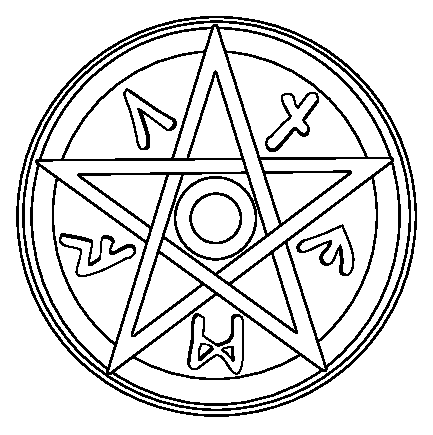
\includegraphics[scale=2]{magus/pentagramma.eps}

\vspace{3em}

{\fontsize{40pt}{0pt}\Aniron{Játékosok}}

{\fontsize{40pt}{0pt}\Aniron{Törvénykönyve}}

\vspace{2em}

\textbf{ÍRTA}

NoiseEHC, Ágasváry

%\textbf{LEKTORÁLTA}

%Éberen Őrködő, wisp

%\textbf{SEGÍTETTE}

\end{center}

\clearpage

\setmainfont[Ligatures=TeX,Scale=1.4]{EB Garamond}

\tableofcontents 

\pagestyle{fancy}
% Ez kikapcsolja, hogy a "...fejezet" szöveg benne legyen a header-ben ("\pagestyle{fancy}" után kell).
\renewcommand{\chaptermark}[1]{\markboth{#1}{}}
\setmainfont[Ligatures=TeX,Scale=1.4]{EB Garamond}

\chapter{Alapok}

A F.A.T.E.M. egy nem hivatalos, rajongói szerepjáték a M.A.G.U.S. világához. A szabályok a \fate{Fate Condensed} játékra épülnek, több helyen kiegészítve azt. Ez egy komplett szerepjáték rendszer; bár pár regényt és világleírást érdemes elolvasnod, nincs más könyvre szükséged a játékhoz.

Ha már itt tartunk, vegyük sorra, hogy mire lesz viszont \emph{tényleg} szükséged!

\section{Mire van szükséged a játékhoz?}

A \fate{Fate Condensed} játékhoz szükséged lesz játékosokra kettő és hat fő között, akikből egy a Kalandmester (KM) szerepét fogja betölteni. Kell még pár kocka, néhány zseton, íróeszközök, papír és még valami a rövid jegyzetekhez (például öntapadó cetlik).

A \fate{Fate Condensed} rendszer \fate{Fate Dobókockákat}™ használ, amikor a karakterek cselekszenek. Ezek hatoldalú kockák, amelyeknek kettő \dice{0}, kettő \dice{+} és kettő \dice{-} oldaluk van. Összesen négy ilyen kocka már elégséges, de a legjobb, ha mindegyik játékos rendelkezik néggyel. Ezen kívül lehet használni standard hat oldalú dobókockát is (1"~2 = \dice{-}, 3"~4 = \dice{0}, 5"~6 = \dice{+}; netán vastagabb filccel át lehet alakítani így:~\vcenteredinclude{d6_to_fudge_v2.png}). Alternatíva még a \fate{Deck of Fate} kártyapakli is, ami kártyalapokat használ dobókockák helyett; ennek ellenére, az egyszerűség kedvéért, a továbbiakban konzekvensen a „dobás” szót használjuk.


\section{Karakterkészítés}

\subsection{Ki vagy valójában?}

Mindegyik játékos egy kalandozót irányít a történetben, meghatározva minden tettüket. Neked kell kidolgoznod a karaktert olyanra, amilyenre szeretnéd. Vedd figyelembe, hogy a Fate karakterek kompetensek, drámaiak, és nem haboznak a kalandokba vetni magukat.

A te JK"~d az alábbi dolgokból épül fel:

\begin{itemize}
    \item \textbf{Jellemzők:} kifejezések, amik leírják, hogy ki is a hősöd
    \item \textbf{Képességek:} megadják, hogy a hősöd miben jobb másoknál
    \item \textbf{Fortélyok:} figyelemre méltó dolgok, amit a hősöd meg tud tenni
    \item \textbf{Stressz:} a hős azon adottsága, hogy nyugodt maradjon, és folytassa küldetését
    \item \textbf{Következmények:} fizikai és szellemi sérülések, amit a hős még elvisel
    \item \textbf{Újratöltés:} ez mutatja a hős narratív hatalmát
    \item \textbf{Végső simítások:} a hős leírásának részletei
\end{itemize}


\clearpage
\subsection[Jellemzők]{Jellemzők (Aspect)}

A \definition{jellemzők} rövid leírók, amik megadják, hogy ki is a karaktered, vagy, hogy mi fontos neki. Kapcsolódhatnak a karaktered testi vagy mentális tulajdonságaihoz, történetéhez, hitéhez, kiképzéséhez, ismeretségeihez vagy akár a különösen fontos felszerelési tárgyaihoz.

A legelső dolog, amit tudni kell róluk, hogy a \textbf{jellemzők mindig igazak} (lásd az értekezést a \onpage{A jellemző mindig igaz}). Más szóval, amit kitalálsz karakterkészítés közben, az mind valóságos és igaz a történetben. Ha leírod, hogy a karakter egy \aspect{Jövőbelátó Mesterlövész}, akkor ő egy jövőbelátó mesterlövész. Ezzel közhírré tetted, hogy a karakter látja a jövőt, és nagyon jó a távcsöves puskával.

A jellemzőkkel meg tudod változtatni játék közben a történetet. Lehetővé teszik, hogy javíts a dobások eredményén, és tényeket kreálhatsz a világban. Végül, a jellemzőkkel \definition{sors pontokat} szerezhetsz, ha komplikációkat okoznak a karakterednek -- így a legsokoldalúbb jellemzők létrehozásához lehetőleg válassz kétélűeket, amik segíthetnek és hátráltathatnak is.

Ha szeretnél többet is megtudni a jellemzőkről, és hogy mi teszi igazán jóvá őket, olvasd el a \textit{„Jellemzők és sors pontok”} fejezetet (\page{Jellemzők és sors pontok}).

\textbf{Kezdetben adj a karakternek öt jellemzőt:} egy koncepciót, egy árnyoldalt, egy kapcsolatot és még kettő szabadon választott jellemzőt. Kezdd az egészet a koncepció jellemzővel.

\subsubsection{Koncepció jellemző (High Concept)}

A \definition{koncepció} a karakter általános leírása, csak a leglényegesebb dolgokat lefedve. Képzeld el, hogy egy ismerősödnek mesélsz a karakterről, és így kezdenéd a történetet.

\subsubsection{Árnyoldal jellemző (Trouble)}

A következő az \definition{árnyoldal}, ami a karakter életének komplikálására szolgál. Ez lehet egy gyengeség, családi kötelék, vagy más kötelezettség. Válassz olyat, amit élveznél eljátszani.

\subsubsection{Kapcsolat jellemző (Relationship)}

A \definition{kapcsolat} összeköti a karakteredet egy másik JK"~val. Lehet, hogy ők már régről ismerték egymást, de az is lehetséges, hogy csak mostanában futottak össze.

Egy kapcsolat jellemző akkor jó, ha magába foglal, vagy utal valami konfliktusra, de legalábbis a kötelék féloldalasságára, ami így dinamikát ad a kapcsolatnak. Ez nem azt jelenti, hogy nyíltan ellenségesek, de az sem a legjobb, ha minden tökéletesen szép és passzol köztük.

Ha neked úgy jobb, várhatsz a kapcsolat jellemzővel, amíg mindenki többé"~kevésbé elkészül a saját karakterével.

\subsubsection{Szabadon választott jellemzők}

A karakter utolsó két jellemzőjének azt választasz, amit csak akarsz -- annyi csak a megkötés, hogy szervesen kell illeszkednie a világba. Válassz olyat, ami szerinted érdekesebbé teszi a karaktered, vagy amitől élvezetesebb lesz eljátszani őt, vagy amitől jobban passzol a világba.

\clearpage
\subsection{Képességek}

Míg a jellemzők megadják, hogy ki a karakter, addig a \definition{képességek} azt mutatják, hogy mit képes megtenni. Minden képesség tevékenységek széles körét foglalja magába, amit a karakter képzés vagy gyakorlás útján sajátított el, netán csak veleszületett. A karakter a Tolvajlás képességgel, valamilyen szinten, bármilyen bűntényt elkövethet, ami a lopás művészetéhez kapcsolódik -- terepszemle, biztonsági rendszer megkerülése, zsebmetszés, zárnyitás.

Minden képességnek van egy \definition{szintje}. Minél magasabb a szint, annál jobb a karakter abban a dologban. A karaktered képességeinek összessége mutatja, hogy mi az, amire született, mi az, amivel még megbirkózik, és mi az, amit nem kéne erőltetnie.

A karaktered képességeinek szintjeit az alábbi piramis struktúra alapján választhatod ki, ahol a legmagasabb szint a Kimagasló~(+4):

\begin{itemize}
    \item Egy darab Kimagasló~(+4) képesség
    \item Kettő darab Remek~(+3) képesség
    \item Három darab Jó~(+2) képesség
    \item Négy darab Átlagos~(+1) képesség
    \item Minden más képesség szintje Középszerű~(+0)
\end{itemize}

\subsubsection{Képesség szintek skálája}

A \fate{Fate Condensed} játékban, ahogy a normális Fate játékban is, a képességek szintjei az alábbi skálába vannak rendezve:

\begin{center}
\fatetable{r l}{
\textcolor{white}{Szint} & \textcolor{white}{Melléknév} \\
+8 & Legendás (Legendary) \\
+7 & Epikus (Epic) \\
+6 & Fantasztikus (Fantastic) \\
+5 & Emberfeletti (Superb) \\
+4 & Kimagasló (Great) \\
+3 & Remek (Good) \\
+2 & Jó (Fair) \\
+1 & Átlagos (Average) \\
+0 & Középszerű (Mediocre) \\
-1 & Gyenge (Poor) \\
-2 & Borzalmas (Terrible) \\
-3 & Katasztrofális (Catastrophic) \\
-4 & Horrorisztikus (Horrifying) \\
}
\end{center}

\clearpage
\subsection{Újratöltés}

Az \definition{újratöltés} megmondja, hogy a karaktered mennyi \definition{sors ponttal} (\page{24}) kezdi a játéküléseket. Alapállapotban a karaktered újratöltése 3.

A sors pontjaid száma minden játékülés elején legalább az újratöltés értéke lesz. Emiatt mindenképpen jegyezd fel, hogy mennyi sors ponttal fejezed be a játékülést -- ha ez több, mint az újratöltésed, akkor a következő játékban annyival fogsz kezdeni.

\example{%
Charles jó sok sors pontot szerzett a játék során, a végére 5 maradt nála. Mivel az ő újratöltése 2, így a következő játékot 5"~el is fogja kezdeni. Ellenben Ethannél csak egyetlen sors pont marad. Az ő újratöltése 3, így a következő játékot 3 sors ponttal fogja kezdeni, nem a megmaradt 1"~el.
}

\subsection{Fortélyok}

Bár minden karakter használhat minden képességet -- még ha a többségüknek Középszerű~(+0) is a szintje -- \definition{fortélyokkal} egyedivé teheted a karakteredet. A fortélyok lehetnek menő vagy titkos technikák, trükkök vagy felszerelések, amik a karaktereket egyedivé és érdekesebbé teszik. Míg egy képesség a karakter hozzáértésének átfogó leírása, addig egy fortély nagyon szűk területen mutatja a kiválóságát; a többségük csak jól meghatározott szituációkban ad bónuszt, vagy tesz lehetővé cselekedeteket, amiket más karakter egyszerűen tud megtenni.

A karakterednek alapértelmezésben három fortély rubrikája lehet. Nem muszáj rögtön karakterkészítéskor kitalálni őket, elég, ha játék közben töltöd ki. Vásárolhatsz több fortélyt is, feláldozva 1 újratöltést mindegyikért, de az újratöltéseid száma nem mehet 1 alá.

\subsection{Kasztok}

Ebben a játékban a kasztok nem kötelezően választandó kategóriák, hanem csak egy ötlet lista, amit felhasználhatsz a karaktered elkészítéséhez. Nem muszáj választanod közülük, de a KM bizonyos -- főleg mágikus -- hatásokat és speciális szabályokat csak bizonyos kasztok tagjainak engedélyez. Ha a karaktered kaszt nélküli, attól még szabadon válogathatsz a fortélyok listájának nagy részéről is.

Egy kaszt felvétele egy jellemző megfelelő elnevezését igényli, erre több példát is adunk. Célszerű, ha a kaszt a karakter koncepció vagy árnyoldal jellemzőinek egyike, de ez nem kötelező. Bizonyos kasztok megkötéseket és kötelezettségeket vonnak maguk után, ezek játék közben késztetésekként jelentkezhetnek.

\subsection{Fajok}

A fajok a kasztokhoz nagyon hasonlóan vannak megvalósítva, de azokkal ellentétben nem variálhatók szabadon. Ha a karakter ember, akkor nem kell egy jellemzőt a fajára elhasználni, és így több jellemző marad az érdekes tulajdonságaira. Ellenben a fajok különböző passzív bónuszokat biztosíthatnak, mivel a jellemző mindig igaz (\page{A jellemző mindig igaz}). A faj kötelezően a karakter koncepció vagy árnyoldal jellemzője legyen!

\clearpage
\subsubsection{Fortélyok megtervezése}

A fortélyokat te találod ki, a karakter kitalálása közben. Nagy vonalakban a fortélyokat két csoportra lehet osztani.

\textbf{Bónuszt adó fortélyok:} A fortélyok első típusa \textbf{+2 bónuszt ad}, amikor egy meghatározott képességet használsz bizonyos határokon belül, általában csak bizonyos cselekvésekhez (\page{Cselekvések}), és bizonyos narratív körülmények között.

Az ilyen fortélyokat az alábbi módon célszerű megfogalmazni:

\example{%
Mivel \textbf{[írd le, hogy mennyire menő a karakter vagy a felszerelése]}, ha a \textbf{[válassz egy képességet]} képességet használom \textbf{[válassz a megoldásra, helyzetbehozásra, megtámadásra, védekezésre közül]}, +2 bónuszt kapok, de csak ha \textbf{[definiáld a körülményeket]}.
}

\textbf{Bónuszt adó fortély példa:} Mivel én egy \textbf{katonai mesterlövész} vagyok, ha a \textbf{Célzás} képességet használom \textbf{megtámadásra}, +2 bónuszt kapok, de csak \textbf{ha a \aspect{Célpont Bemérve}}.

\textbf{Szabályszegő fortélyok:} A fortélyok második típusa \textbf{megváltoztatja a játék szabályait}. Ez egy átfogó kategória, amibe az alábbiak mind beletartoznak, de kitalálhatsz mást is:

\begin{itemize}
    \item \textbf{Megváltoztatni, hogy melyik képességet kell használni bizonyos szituációkban.} Például egy kutató használhat Tudományt egy rituálé elvégzéséhez, míg mindenki más Misztikumot.
    \item \textbf{Olyan cselekvést végezni egy képességgel, ami normálisan nem lehetséges.} Például, hogy egy karakter hátba szúrjon egy ellenfelet az árnyékokból a Lopózás képességgel, míg normálisan ez megtámadás cselekvés lenne a Közelharc képességgel.
    \item \textbf{Nagyjából +2 értékű, nem számszerű bónuszt adni egy képesség használatához.} Például, ha egy tehetséges szónok Befolyásolással helyzetbe hoz, kap egy extra ingyen kihasználást.
    \item \textbf{Megengedni, hogy a karakter kinyilváníthasson egy kisebb tényt, ami igazzá válik.} Például egy túlélésben képzett karakternél mindig legyen pár túléléshez szükséges eszköz, mint mondjuk gyufa, még akkor is, ha ez nagyon valószínűtlen is a történetben. Ez a fortély fajta lehetővé teszi, hogy a történet részleteinek kinyilvánítása (\page{Történet részleteinek kinyilvánítása}) jellemző kihasználása nélkül is elérhető legyen.
    \item \textbf{Megengedni, hogy a karakter megszeghessen pár szabályt.} Például a karakter kaphat két extra stressz dobozt vagy egy extra enyhe következmény rubrikát.
\end{itemize}

Az ilyen fortélyokat az alábbi módon célszerű megfogalmazni:

\example{%
Mivel \textbf{[írd le, hogy mennyire menő a karakter vagy a felszerelése]}, képes vagyok \textbf{[írj le egy bámulatos tettet]}, de csak \textbf{[definiáld a körülményeket vagy korlátokat]}.
}

\textbf{Szabályszegő fortély példa:} Mivel \textbf{nem hiszek a mágiában}, képes vagyok \textbf{természetfeletti adottságok hatásait figyelmen kívül hagyni}, de csak \textbf{játékülésenként egyszer}.

\clearpage
\subsection{Stressz dobozok és következmény rubrikák}

A \definition{stressz dobozok} és a \definition{következmény rubrikák} adják meg, hogy a karakter mennyire tudja tolerálni a fizikai és szellemi igénybevételt a kalandok során. Minden karakternek legalább 3, egy"~egy pontot érő fizikai stressz doboza, és legalább 3, egy"~egy pontot érő szellemi stressz doboza van. Szintén van egy"~egy enyhe, mérsékelt és súlyos következmény rubrikája.

A Fizikum képesség szint módosítja, hogy a karakternek mennyi fizikai következmény rubrikája van. Az Akaraterő ugyanígy hat a szellemi következmény rubrikák számára.

\begin{center}
\fatetable{l l}{
\textcolor{white}{Fizikum/Akaraterő} & \textcolor{white}{Fizikai/Szellemi stressz} \\
Középszerű~(+0) & \dice{3} \\
Átlagos~(+1) vagy Jó~(+2) & \dice{31} \\
Remek~(+3) vagy Kimagasló~(+4) & \dice{33} \\
Emberfeletti~(+5) vagy magasabb & \begin{tabular}[t]{@{}l@{}}\dice{33}\\és egy extra enyhe következmény rubrika,\\specifikusan csak a fizikai\\vagy csak a szellemi sérülésekre\end{tabular} \\
}
\end{center}

A \textit{„Sérülések elszenvedése”} fejezetben (\page{34}) többet is tanulhatsz a stresszről és következményekről.

\subsubsection{Várjunk csak, nem erre emlékszem!}

A \fate{Fate Condensed} szabályokban minden stressz doboz csak 1 pontot ér. Ellenben a \fate{Fate Core} és a \fate{Fate Accelerated} rendszerekben a stressz dobozok értéke növekvő (1 darab 1 pontos, 1 darab 2 pontos, és így tovább). Használhatod azt a rendszert is, ha úgy tetszik; mi azért váltottunk az 1 pontos dobozokra, mert egyszerűbb -- a másik módszer egy kicsit könnyebben összezavarja az embereket.

Ennek a stílusnak viszont van pár folyománya, amit jó lesz észben tartani.

\begin{itemize}
    \item Ahogy azt majd a \onpage{35} láthatod, az 1 pontos dobozokból annyit ikszelsz be, amennyit csak akarsz, ha találatot kapsz (míg a növekvő értékű dobozokból mindig csak egyet lehetett).
    \item Ehhez a stílushoz különálló fizikai és szellemi stresszmérők szükségesek, ellentétben a \fate{Fate Accelerated} rendszer közös stresszmérőjével. Ha a közös stresszmérő jobban tetszik, akkor adj hozzá három dobozt kiegyenlítésként, és használd a magasabb szintűt a Fizikum és Akaraterő közül, hogy megnöveld a számukat.
    \item Három pontnyi stressz semlegesítés nem túl sok! Ha a karakterek egy kissé törékenynek tűnnének játék közben, nyugodtan adjál hozzá egy"~két dobozt az alapértelmezetthez mennyiséghez. Ez az egész csak annyiról szól, hogy milyen gyorsan váltunk következményekre. (A régebbi rendszerben egy \boxed{1}~\boxed{2} sorozat 2"~3, egy \boxed{1}~\boxed{2}~\boxed{3} sorozat 3"~6, míg egy \boxed{1}~\boxed{2}~\boxed{3}~\boxed{4} sorozat 4"~10 stresszt semlegesített.)
\end{itemize}

\subsection{Végső simítások}

Nevezd el a karaktert, írd le, hogy hogyan néz ki, és beszéld meg a múltját a többi játékossal. Ha még nem írtad le a kapcsolat jellemzőt, akkor itt az ideje megtenni.

\clearpage

\label{Cselekedni}
\chapter{Cselekedni és kockákkal dobni}

A \fate{Fate Condensed} játékban te irányítod a karaktered cselekedeteit, miközben hozzáteszel a közösen mesélt történethez. Általában a KM meséli, hogy a világban mi történik, és hogy a Nem Játékos Karakterek (\definition{NJK}"~k) mit csinálnak, míg a játékosok a saját karaktereik cselekedeteit mondják el.

Bármit szeretnél csinálni, kövesd az \definition{előbb az elképzelés} szabályt: először mondd ki, hogy a karaktered mire készül, és csak \emph{utána} gondolkodj azon, hogy a rendszerben ezt hogyan lehet modellezni. A karaktered jellemzői megmutatják, hogy mivel próbálkozhat egyáltalán, és segítenek megállapítani az eredmény értelmezésének kereteit. A legtöbb ember meg sem próbálkozhat megműteni a kibelezett társát, de ha van egy jellemződ, ami orvosi háttérről árulkodik, akkor te viszont nekiláthatsz. Enélkül a jellemző nélkül a legtöbb, hogy nyerhetsz pár percet a végső szavakhoz. Ha kétségesnek érzed, kérdezd meg a KM"~et és az asztaltársaságot.

Hogyan állapítod meg, hogy eredményes voltál"~e? Gyakran a karaktered egyszerűen csak megteszi, amit akartál, mert a cselekedet nem túl nehéz, és senki sem próbált meggátolni benne. De problémás és kiszámíthatatlan szituációkban muszáj elővenni a kockákat, hogy eldöntsék, mi történik.

Ha egy karakter cselekedne, az alábbiakat kell figyelembe venni:

\begin{itemize}
    \item Mi gátolja abban, hogy egyszerűen csak megtegye?
    \item Mi mehet félre?
    \item Miért érdekes, ha valami félresikerül?
\end{itemize}

Ha senkinek sincs megfelelő válasza az összes kérdésre, akkor a cselekedet egyszerűen megtörténik. Elvezetni a repülőtérre tényleg nem kíván kockadobálást. Viszont az autópályán versenyezni a ránk várakozó repülőig, miközben másik világról származó, kibernetikával turbózott vadállatok üldöznek, tökéletes alkalom a dobásra.

Ha cselekedni kívánsz, kövesd az alábbi lépéseket:

\begin{enumerate}
    \item Előbb az elképzelés: írd le, mit akarsz megtenni, és utána válassz képességet és cselekvést.
    \item Dobj négy kockával.
    \item Add össze a szimbólumokat a kockákon: a \dice{+} értéke +1, a \dice{-} értéke -1, míg a \dice{0} értéke 0. Ez -4~és~+4 közötti eredményt fog adni.
    \item Add a kockák eredményét a képesség szintjéhez.
    \item Módosíthatod a dobást jellemzők kihasználásával (\page{Jellemzők kihasználása} és \page{Kihasználás}) és fortélyok használatával (\page{Fortélyok használata}).
    \item Állapítsd meg a végső eredményt, aminek a neve \definition{erőfeszítés}.
\end{enumerate}

\clearpage
\label{Nehézség és ellenállás}
\section{Nehézség és ellenállás}

Ha a karakter tettét valamilyen probléma akadályozza, vagy pedig egy másik karakter vagy lény helyett csak a világra próbál hatni, akkor a cselekvésének passzív \definition{nehézséget} kell legyűrnie. Ilyen például a zártörés, ajtók eltorlaszolása vagy felmérni az ellenség táborát. A KM változtathat a nehézségen, ha ezt bizonyos jellemzők (legyenek azok a karakteren, a jeleneten vagy máshol) indokolják.

Más esetekben, az ellenfél aktív \definition{ellenállást} tanúsít a karakter cselekvésével szemben egy védekezés cselekvést használva (\page{Védekezés}). Ezekben az esetekben a KM szintén dob, ugyanazokat a lépéseket követve az előző fejezetből, miközben az ellenfél képességeit, fortélyait és jellemzőit használja. Ha megtámadásra vagy az ellenfelet közvetlenül érintő helyzetbehozásra dobsz, az ellenfél védekezésre fog dobni ellene.

Az ellenállásnak számtalan formája létezik. Ha egy szektataggal a rituális áldozótőrért küzdesz, akkor az ellenfél jól definiált. De lehetséges, hogy egy ősi rituálé erejével kell megküzdened, hogy meg tudd menteni a világot. Feltörni egy széfet a First Metropolitan Bank páncéltermében a felfedezés kockázatát hordozza, de az a KM döntése, hogy a járőröző őrség aktív \emph{ellenállása} ellen dobsz, vagy pedig csak a széftől függő passzív \emph{nehézség} ellen.

\section{A dobás módosítása}

Kihasználhatsz egy jellemzőt, hogy +2 bónuszt kapjál a dobásra, vagy pedig újra dobhass. Néhány fortély szintén bónuszokat adhat. A jellemzők kihasználásával egy szövetségesedet is támogathatod (\page{Csapatmunka}), vagy az ellenfél dobásának nehézségét is megnövelheted.

\label{Jellemzők kihasználása}
\subsection{Jellemzők kihasználása}

Ha csinálsz valamit, de a kockák eredménye nem elégséges, nem kell feladnod, és elfogadni a vereséget. (Bár nyilvánvalóan megteheted. Az is lehet mókás.) A használható jellemzők opciókat és lehetőségeket biztosítanak ahhoz, hogy elérd a célod.

Ha meg tudod indokolni, hogy egy jellemző hogyan segíthet a fáradozásaidban, fogalmazd meg, hogyan segít, és költs el egy sors pontot a \definition{kihasználásához} (vagy használj el egy ingyen kihasználást). Hogy mi indokolható meg, és mi nem, annak eldöntésére a \definition{fals szabály} szolgál -- bárki megvétózhatja, ha kijelenti, hogy „Ez fals!”. Egyszerűen fogalmazva, a fals szabály \textbf{kalibrációs technika}, amit minden jelenlévő használhat, ha úgy érzi, hogy a játék eltávolodott a megcélzott víziótól vagy koncepciótól. Hasonló technikákról, amik a biztonságos játékkörnyezet kialakítását célozzák, a \onpage{Biztonsági technikák} olvashatsz.
Ha a kihasználásod falsnak bizonyul, két lehetőséged van. Először is, visszavonhatod a kihasználást, és próbálkozhatsz mással, például egy másik jellemzővel. Másodszor, megvitathatod, hogy a jellemző miért is megfelelő. Ha ez nem győzi meg a másikat, akkor vond vissza a kihasználást, és nyugodj bele. Ha magáévá teszi a perspektívádat, akkor viszont csinálhatod a kihasználást, ahogy tervezted. A fals szabály arra szolgál, hogy az asztal mellett töltött idő kellemesen teljen. Akkor használd, ha valami nem hangzik túl jól, nincs sok értelme, vagy nem illik a megcélzott hangulatba. Ha valaki kihasználná a \aspect{Nagyszerű Első Benyomás} képességét, hogy eldobjon egy autót, az valószínűleg fals. De lehetséges, hogy van a karakternek valamilyen természetfeletti jellemzője, ami elképzelhetetlenül erőssé teszi, elég erőssé, hogy eldobjon egy autót, és ez a belépő egy rettentő szörnyeteg elleni harcban. Ez esetben a \aspect{Nagyszerű Első Benyomás} teljes mértékben hihető.

Amikor kihasználsz egy jellemzőt, vagy \textbf{+2 bónuszt kapsz} az erőfeszítésre, vagy \textbf{újradobhatod mind a négy kockát}, vagy pedig \textbf{2"~vel emelheted a nehézséget} valaki más dobásánál, ha ez megmagyarázható. Több jellemzőt is kihasználhatsz ugyanahhoz a dobáshoz, de nem lehet kihasználni ugyanazt a jellemzőt többször ugyanahhoz a dobáshoz. Az egyetlen kivétel: tetszőleges számú \emph{ingyen kihasználásod} elhasználhatod ugyanazzal a jellemzővel ugyanahhoz a dobáshoz.

Kihasználni legtöbbször a saját karaktered jellemzőit fogod. De kihasználhatsz helyzet jellemzőket is, sőt, lehetőség van más karakter jellemzőinek ellenséges kihasználására is (\page{Ellenséges kihasználás}).

\label{Fortélyok használata}
\subsection{Fortélyok használata}

A fortélyok bónuszt adhatnak a dobásra, feltéve, hogy teljesíted a fortély leírásában megfogalmazott feltételt, például a megfelelő körülményeket, a használt cselekvést vagy képességet. Használhatod a helyzetbehozás cselekvést is (\page{Helyzetbehozás}, hogy olyan jellemzőket hozzál létre, amik megteremtik a fortélyhoz szükséges körülményeket. Végül, vedd figyelembe a fortély szükséges körülményeit a karaktered cselekedeteinek leírásakor is, hogy ennyivel is könnyebb legyen a feltételeket teljesítened.

Normális esetben a fortély +2 bónuszt ad, egy bizonyos, szűken definiált szituációban, bármiféle költség nélkül; bármikor használhatod, amikor csak lehetséges. Ellenben, néhány ritka és kivételesen hatalmas fortélyhoz lehet, hogy el kell költened egy sors pontot a használathoz.

\label{Kimenetelek}
\section[Kimenetelek]{Kimenetelek (Outcome)}

Minden dobás után az erőfeszítés, valamint a passzív nehézség vagy aktív ellenállás közötti különbséget a \definition{sikerességnek} hívjuk. Négyféle lehetséges kimenetel létezik:

\begin{itemize}
    \failureitem Ha az erőfeszítés kisebb, mint a megcélzott nehézség vagy ellenállás, akkor \textbf{kudarc}.
    \tieitem Ha az erőfeszítés egyenlő a céllal, akkor \textbf{döntetlen}.
    \successitem Ha az erőfeszítés egy vagy kettő sikerességgel nagyobb, mint a cél, akkor \textbf{siker}.
    \successwithstyleitem Ha az erőfeszítés legalább három sikerességgel nagyobb, mint a cél, akkor \textbf{átütő siker}.
\end{itemize}

Némelyik kimenetel nyilvánvalóan jobban esik, mint mások, de valamilyen érdekes módon mindegyiküknek előre kell mozdítani a történetet. Az előbb az elképzelés szabállyal kezdted (\page{Cselekedni}), hát fejezd is be vele, hogy a történet maradjon a játék fókusza, és hogy a kimenetel értelmezése megfeleljen az elképzelésnek.

\example{%
Ethan nem valami ügyes mackós (bár megvannak hozzá a szerszámai), de mégis ott találjuk a vészjósló kultusz titkos főhadiszállásán, és már csak egy páncélajtó választja el a keresett rituálé kötettől. Át tud"~e jutni rajta?
}

\newpage

\outcomesection{Kudarc}{Kudarc (Failure)}{Ha az erőfeszítés kisebb, mint a megcélzott nehézség vagy ellenállás, akkor kudarcot vallasz.}

Ezt többféleképpen is ki lehet játszani: egyszerűen kudarc, siker komoly áron, vagy elszenvedni egy találatot.

\subsubsection{Egyszerű kudarc}

Az elsőt a legegyszerűbb megérteni -- \definition{egyszerűen kudarc}. Nem éred el a célod, nem haladsz előre, nem kapsz semmit sem. Ez viszont mindenképpen mozdítsa előre a történetet -- ha a széfet egyszerűen csak nem tudod kinyitni, az sehová sem vezet, és unalmas is.

\example{%
Ethan diadalmasan meghúzta a kart, de a széf határozottan zárva maradt, ellenben a szirénák felharsantak. A kudarc megváltoztatta a szituációt, és előremozdította a történetet -- az őrök már a helyszínre tartanak. Ethannek egy újabb dilemmával kell szembenéznie -- most, hogy a finom módszerek sikertelennek bizonyultak, próbálja más módon kinyitni a széfet, vagy hagyja a fenébe, és tűnés?
}

\label{Siker komoly áron}
\subsubsection{Siker komoly áron}

A második a \definition{siker komoly áron}. Megteszed, amit akartál, de komoly árat kell fizetni érte -- a szituáció rosszabbodott, de legalábbis komplikációk léptek fel. Mint KM, egyszerűen kijelentheted, hogy ez lett a kimenetel, vagy pedig felajánlhatod a játékosnak, mint opciót a kudarc helyett. Mindkét variáns jó és hasznos lehet a megfelelő szituációban.

\example{%
Ethan elrontja a dobását, és a KM így szól: „Hallod, ahogy az utolsó retesz a helyére kattan. Ez a hang szinte visszhangzik egy felhúzott revolver kattanásában, ahogy az őr megkér, hogy fel a kezekkel.” A komoly ár itt a konfrontáció az őrrel, amit a karaktere megpróbált elkerülni.
}

\subsubsection{Elszenvedni egy találatot}

Végül, \definition{elszenvedhetsz egy találatot}, amit vagy stressz dobozokkal vagy következményekkel kell semlegesítened, vagy valami más hátrányban részesülhetsz. Ilyen kudarc a leggyakrabban megtámadás elleni védekezés közben fordul elő, vagy ha a karakter megoldana veszélyes problémákat. Annyiban különbözik az egyszerű kudarctól, hogy egyedül a karaktert érinti, nem az egész csapatot. A siker komoly áron annyiban más, hogy itt a siker nem feltétlenül lehetséges.

\example{%
Ethan kinyitja a széfet, de ahogy megfogja a fogantyút, egy szúrást érez a kézfején. Nem hatástalanította a csapdát! Beírja, hogy Megmérgezett az enyhe következmény rubrikába.
}

Ezeket a lehetőségeket keverni is lehet. Az ártalmas kudarc kicsit durvának tűnhet, de lehet, hogy a legjobb választás abban a pillanatban. Vagy a siker találat árán is egy opció.

\newpage

\outcomesection{Döntetlen}{Döntetlen (Tie)}{Ha az erőfeszítés egyenlő a megcélzott nehézséggel vagy ellenállással, az döntetlen.}

A kudarchoz hasonlóan a döntetlennek is előre kell mozdítania a történetet, sosem akadályozhatja az akciót. Muszáj valami érdekesnek történnie. Ugyanúgy, ahogy a kudarc esetén, ezt is többféleképpen ki lehet játszani: siker kisebb áron vagy részleges siker.

\label{Siker kisebb áron}
\subsubsection{Siker kisebb áron}

Az első a \definition{siker kisebb áron} -- pár doboznyi stressz, valamiféle kényelmetlenség vagy hátráltatás a történetben, amik azért magukban nem akadályoznak, netán egy előny jellemző (\page{Előny jellemzők}) az ellenfélnek mind"~mind kisebb árnak számítanak.

\example{%
Ethan kezdeti próbálkozásai mind hibásnak bizonyulnak. Mire kinyitja a széfet, már hajnal hasadt, így szóba se jöhet, hogy az éj leple alatt tűnjön el. Megszerezte, amiért jött, de a szituáció már kellemetlenebb.
}

\subsubsection{Részleges siker}

A döntetlen kezelésének másik módja a \definition{részleges siker} -- ez siker, de csak egy részét tudtad elérni a célodnak.

\example{%
Ethan éppen csak résnyire tudja kinyitni a páncélajtót -- ha csak egy ujjnyival megmozdítaná, a riasztás megszólalna, és fogalma sincs, hogyan tudná hatástalanítani. Pár oldalnyit a rituáléból ki tud húzni a résen át, de csak találgathat a befejező lépésekről.
}

\outcomesection{Siker}{Siker (Success)}{Ha az erőfeszítés eggyel vagy kettővel nagyobb a célnál, az siker.}

Megszerzed, amit akarsz, bármiféle extra fizetség nélkül.

\example{%
Kinyílt! Ethan felmarkolja a rituálé szövegét, és elillan, mielőtt az őrök felfedezhetnék.
}

\subsubsection{Az „előbb az elképzelés” hatása a sikerre}

Az elképzelés \emph{mondja meg}, hogy pontosan hogyan is néz ki a siker. Mi van, ha Ethannek nincsenek szerszámai, vagy nem elég képzett, hogy feltörje a széfet? Ilyenkor lehetséges, hogy a siker inkább „kisebb áron” fog történni. Hasonlóan, ha Ethan azért volt a betörő csapatban, mert ő \emph{építette} a széfet, akkor a siker eléggé „átütő” lesz.

\outcomesection{Átütő siker}{Átütő siker (Success With Style)}{Ha az erőfeszítés legalább hárommal nagyobb a célnál, az átütő siker.}

Megszerzed, amit akarsz, és még egy kicsit többet is.

\example{%
Ethan több mint szerencsés; a széf ajtaja szinte rögtön kinyílik. Nem csak, hogy megszerzi a rituálé szövegét, de elég ideje van átfutni a széfben lévő többi dokumentumot is. Mindenféle váltók és szerződések között rábukkan az Akeley kastély tervrajzára.
}

\clearpage
\label{Cselekvések}
\section[Cselekvések]{Cselekvések (Actions)}

Négyféle cselekvés van, amire dobhatsz, mindegyik egyedi céllal rendelkezik, és egyedi a hatása is a történetre:

\begin{itemize}
    \item \textbf{Megold} egy problémát, hogy leküzdjön egy akadályt a képességeivel.
    \item \textbf{Helyzetbehozás}, hogy előnyösebbé változtassa a körülményeket.
    \item \textbf{Megtámadás}, ami az ellenfélnek kárt okoz.
    \item \textbf{Védekezés}, hogy megússzon egy megtámadást, megállítsa az ellenfelek helyzetbehozását, vagy szembeszegüljön egy probléma megoldásának.
\end{itemize}

\label{Megoldás}
\actionsection{O}{Megoldás}{Megoldás (Overcome)}{Megold egy problémát, hogy legyőzzön egy akadályt a képességeivel.}

Minden karakter számtalan kihívással szembesül a történetben. A \definition{megold} cselekvéssel tudnak szembeszegülni, és legyőzni ezeket az akadályokat.

Egy karakter, akinek magas az Atléta képessége, fel tud mászni a falakon, vagy a zsúfolt utcákon rohanni. Egy detektív magas Nyomozással olyan nyomokat is értelmezhet, ami felett mások átsiklottak. Ha valaki képzett Befolyásolásban, sokkal könnyebben elkerülheti a verekedést egy ellenséges bárban.

A megoldás kimenetelei:

\begin{itemize}
    \failureitem \textbf{Ha kudarc,} beszéld meg a KM"~el (és a védekező játékossal, ha van ilyen), hogy ez egyszerű kudarc, netán siker komoly áron (\page{Siker komoly áron}).
    \tieitem \textbf{Ha döntetlen,} akkor ez egy siker kisebb áron (\page{Siker kisebb áron}) -- kellemetlen szituációba kerülsz, az ellenfél kap egy előny jellemzőt (\page{Előny jellemzők}), vagy elszenvedsz egy találatot. Alternatíva, ha kudarcot vallasz, de kapsz egy előnyt.
    \successitem \textbf{Ha siker,} akkor eléred a célod, és a történet megy tovább, bármiféle bukkanó nélkül.
    \successwithstyleitem \textbf{Ha átütő siker,} akkor nem csak, hogy siker, de kapsz egy előnyt is.
\end{itemize}

\example{%
Charles eljutott az Antarktiszra a kutató létesítményhez. Az épületek romokban, és a lakók sehol. Át akarja kutatni a törmeléket nyomok reményében. A KM azt mondja, hogy dobjon Nyomozásra Jó~(+2) nehézség ellen. Charles dobása \dice{00++} a kockákon, plusz a Nyomozása Átlagos~(+1), az erőfeszítés így Remek~(+3). Ez siker! A KM leírja a nyomokat: lábnyomok a hóban, olyan lényeké, amik sok vékony, nem emberi lábakon lépkednek.
}

Gyakran használjuk a megold cselekvést, ha el kell dönteni, hogy a karakter hozzáfér"~e, vagy észrevesz"~e egy bizonyos tényt vagy nyomot. Ha így van, tartsd észben, hogy létezik a siker valamilyen áron lehetőség is. Ha megakasztaná a történetet, hogy ha egy részlet felett elsiklanának a játékosok, akkor legjobb ezt a lehetőséget teljesen kizárni, és csak az árra fókuszálni.

\newpage

\label{Helyzetbehozás}
\actionsection{C}{Helyzetbehozás}{Helyzetbehozás (Create An Advantage)}{Létrehoz egy új helyzet jellemzőt, vagy a maga javára fordít egy már meglévő jellemzőt.}

A \definition{helyzetbehozás} cselekvéssel a történet folyását tudod megváltoztatni. A képességeiddel új jellemzőket behozva, vagy meglévő jellemzőkhöz kihasználásokat adva, magad és a csapattársaid felé billentheted a mérleg nyelvét. Megváltoztathatod a körülményeket (eltorlaszolni egy ajtót vagy előkészülni egy tervvel, aminek a végrehajtására jár ingyen kihasználás), új információkat fedezhetsz fel (kikutatni egy szörny gyenge pontját), vagy felhasználhatsz valami köztudottat (például a CEO kedvenc whisky márkáját).

A helyzetbehozással létrehozott jellemző ugyanúgy működik, mint bármelyik másik: lefekteti a történet körülményeit, ami lehetővé teheti, megakadályozhatja, vagy csak gátolhatja bizonyos cselekedetek végrehajtását -- például nem lehet egy varázslatot elolvasni, ha a szoba \aspect{Töksötét}. Ugyanúgy lehet kihasználni (\page{Kihasználás}), és ugyanúgy késztethet (\page{Késztetés}). Ezen felül egy helyzet jellemző létrehozásakor kapsz hozzá egy vagy több \definition{ingyen kihasználást} is. Az ingyen kihasználás, ahogy azt a neve is mutatja, ingyenes, nem kell érte sors pontot fizetni. Akár még a szövetségeseidnek is átengedheted az ingyen kihasználást.

Ha helyzetbehozásra dobsz, el kell döntened, hogy új jellemzőt hozol létre, vagy egy már meglévőnek szeretnéd hasznát venni. Ha az előbbi, akkor ezt a jellemzőt egy szövetségeshez, ellenséghez vagy a környezethez szeretnéd csatolni? Ha egy ellenségre, akkor az védekezés cselekvést tehet ellene. Egyéb esetekben általában egy nehézség ellen kell ilyenkor dobni, de a KM dönthet úgy is, hogy valaki megpróbál meggátolni, és akkor az védekezés dobás lesz.

A kimenetelek új jellemző létrehozásánál:

\begin{itemize}
    \failureitem \textbf{Ha kudarc,} akkor nem tudod létrehozni a jellemzőt (egyszerű kudarc), vagy létrejön, de az ellenfél kapja az ingyen kihasználást (siker komoly áron). Ez utóbbi esetben a jellemzőt lehet, hogy át kell fogalmazni, hogy az ellenfelet segítse. Még így is megérheti, mert a jellemző mindig igaz (\page{A jellemző mindig igaz}).
    \tieitem \textbf{Ha döntetlen,} akkor nem tudod létrehozni a jellemzőt, de helyette kapsz egy előnyt (\page{Előny jellemzők}).
    \successitem \textbf{Ha siker,} akkor létrehozod a jellemzőt, és kapsz egy ingyen kihasználást.
    \successwithstyleitem \textbf{Ha átütő siker,} akkor létrehozod a jellemzőt, és kapsz \emph{két} ingyen kihasználást.
\end{itemize}

A kimenetelek meglévő, ismert vagy ismeretlen jellemző esetén:

\begin{itemize}
    \failureitem \textbf{Ha kudarc,} és a jellemző ismert volt, akkor az ellenfél kap egy ingyen kihasználást a jellemzőhöz. Ha ismeretlen volt, akkor felfedhetik egy ingyen kihasználásért cserébe.
    \tieitem \textbf{Ha döntetlen,} kapsz egy előnyt, ha a jellemző ismeretlen volt; és ismeretlen is marad. Ha a jellemző ismert volt, akkor ehelyett kapsz egy ingyen kihasználást hozzá.
    \successitem \textbf{Ha siker,} akkor kapsz egy ingyen kihasználást a jellemzőhöz, felfedve, ha addig ismeretlen volt.
    \successwithstyleitem \textbf{Ha átütő siker,} két ingyen kihasználást kapsz a jellemzőhöz, felfedve, ha addig ismeretlen volt.
\end{itemize}

\newpage

\example{%
Ethan szembekerül egy shoggothal, ami egy masszív, fáradhatatlan húshegy. Tisztában van vele, hogy ez túl hatalmas szörny egy direkt megtámadáshoz, ezért úgy dönt, hogy inkább elvonja a figyelmét: „Készítek egy Molotov koktélt, és lángba borítom” -- mondja.
\newline
A KM úgy dönt, hogy a shoggothot triviális eltalálni, ezért ez egy Ezermester dobás lesz -- milyen gyorsan tud találni valami gyúlékonyat, amit fegyverré alakíthat. A nehézség Remek~(+3). Ethan Ezermester képessége Átlagos~(+1), a dobása \dice{0+++}, így az erőfeszítés Kimagasló~(+4).
\newline
Ethan összeüt egy Molotov koktélt, és a szörnyre hajítja. A shoggoth így \aspect{Lángol}, és Ethannek van egy ingyen kihasználása ehhez a jellemzőhöz. Ez láthatóan elvonta a shoggoth figyelmét, így ha üldözni kezdi, Ethan kihasználhatja a jellemzőt, hogy egérutat nyerjen.
}

\label{Megtámadás}
\actionsection{A}{Megtámadás}{Megtámadás (Attack)}{Megtámadja az ellenfelet, hogy kárt okozzon neki.}

A \definition{megtámadás} cselekvéssel lehet megpróbálni kiejteni az ellenfelet -- legyen szó egy undorító szörnyeteg levágásáról, vagy csak egy ártatlan őr kupán vágásáról, aki még csak azt sem tudja, hogy mit őriz. Egy megtámadás lehet egy géppuska ellenfélre ürítése, egy kemény jobb egyenes, netán egy káros varázslat.

Vedd figyelembe, hogy egyáltalán lehetséges"~e sérülést okozni a célpontnak. Nem minden megtámadás hasonló nagyságrendű, egy kaiju valószínűleg meg sem érezné, ha behúznál neki egyet. Döntsd el, hogy a megtámadásnak egyáltalán van"~e reális esélye a károkozásra, mielőtt nekiállnál dobni. Vannak olyan hatalmas lények, amiknek valamilyen gyengeségét kell kiaknázni, vagy a védelmüket kell valahogy megkerülni, mielőtt bármiféle kárt tudnál tenni bennük.

A kimenetelek megtámadás esetén:

\begin{itemize}
    \failureitem \textbf{Ha kudarc,} akkor nem tudod eltalálni -- a támadást kivédték, elmozdultak előle, vagy csak felfogta a páncél.
    \tieitem \textbf{Ha döntetlen,} akkor éppen csak súrolod, vagy talán az ellenfél meghátrált. Akárhogyan is, de kapsz egy előnyt (\page{Előny jellemzők}).
    \successitem \textbf{Ha siker,} akkor a sikerességgel megegyező nagyságú sérülést okozol. A védekező félnek ezt kell stressz dobozokkal vagy következmény jellemzőkkel semlegesítenie, vagy kiejtődik (\page{Kiejtés}).
    \successwithstyleitem \textbf{Ha átütő siker,} akkor ugyanúgy sérülést okozol, mint siker esetében, de választhatod, hogy eggyel kisebb sikerességért, egy extra előnyt is kapsz.
\end{itemize}

\example{%
Ruth belebotlik egy csontvázba, amit misztikus erők állítottak valami sötét dolog szolgálatába. Úgy dönt, hogy orrba vágja. A Közelharc képessége Kimagasló~(+4), de a dobása \dice{-{}-00}, így az erőfeszítés csak Jó~(+2).
}

\newpage

\label{Védekezés}
\actionsection{D}{Védekezés}{Védekezés (Defend)}{Védekezik, hogy megússzon egy megtámadást, vagy meggátolja valaki más cselekvését.}

Egy szörny próbál szétmarcangolni? Egy ellenfél próbál félretaszítani, a haragod elől menekülve? Mit teszel, ha egy szektatag próbálja mindkét veséd szétszurkálni? \definition{Védekezés}, védekezés, védekezés.

A védekezés az egyetlen reakció cselekvés a \fate{Fate Condensed} játékban. A védekezéssel meggátolhatsz valamit, még ha nem is te jössz, így passzív nehézség helyett, gyakran aktív ellenállás dobás lesz. Az ellenséged dob, és rögtön ezután lehetőséged van dobni, ha te vagy a célpont, vagy pedig indokolható, hogy miként tudsz közbeavatkozni (ami gyakran téged tesz célponttá). Néhány jellemző vagy fortély adhat is indoklást.

A kimenetelek védekezés esetén:

\begin{itemize}
    \failureitem \textbf{Ha kudarc} megtámadás ellen, akkor elszenveded a találatot, amit köteles vagy stressz dobozokkal vagy következmény jellemzőkkel semlegesíteni (\page{Stressz}). Más esetben az ellenfeled sikeres abban, amit eltervezett.
    \tieitem \textbf{Ha döntetlen,} az ellenfeled cselekvésének a döntetlen kimenetele adja meg, mit kell tenni.
    \successitem \textbf{Ha siker,} akkor nem szenveded el a találatot, vagy meggátolod az ellenfelet a tervében.
    \successwithstyleitem \textbf{Ha átütő siker,} akkor nem szenveded el a találatot, vagy meggátolod az ellenfelet a tervében, és egy előnyt is kapsz, mert pillanatnyilag felülkerekedtél rajta.
\end{itemize}

\example{%
Az előbbi példát folytatva, a csontváz védekezhet Ruth ellen. A KM dobása \dice{-00+}, ami nem módosítja a lény Középszerű~(+0) Atléta képességét.
\newline
Mivel Ruth erőfeszítése a magasabb, a támadása siker. A sikeresség kettő, és a csontváz egy kicsit közelebb került ahhoz, hogy ne keljen fel megint. Ha a csontváz jobbat dobott volna, akkor a védekezése siker lehetett volna, és az élőhalott szörnyűség elkerülhette volna a találatot.
}

\subsubsection{Mely képességekkel lehet megtámadni és védekezni?}

Az alapértelmezett képesség lista az alábbi elveket követi:

\begin{itemize}
    \item Közelharc és Célzás alkalmas fizikai megtámadásra.
    \item Atlétával bármilyen fizikai megtámadás ellen lehet védekezni.
    \item Közelharccal csak Közelharci megtámadás ellen lehet védekezni.
    \item Kényszerítés alkalmas szellemi megtámadásra.
    \item Akaraterővel lehet szellemi megtámadás ellen védekezni.
\end{itemize}

Speciális körülmények között, más képességeket is lehet megtámadásra vagy védekezésre használni, ha a KM engedélyezi, vagy konszenzus alakul ki a játékosok között. Némelyik fortély adhat szélesebb körű, garantált engedélyt akkor is, amikor a körülmények nem lennének alkalmasak. Ha egy képesség nem használható direkt megtámadásra vagy védekezésre, de hasznos lehet a szituációban, akkor használd a helyzetbehozás cselekvést, és használd el az ingyen kihasználásokat a következő megtámadás vagy védekezés dobásodhoz.

\clearpage

% Itt azért vannak a képességek szétszedve 3 listára, hogy ne foglaljanak túl sok tartalomjegyzéket, de azért még meg lehessen őket találni.
\chapter{Képesség lista}
\section{Fizikai képességek}
\engskill{Atléta}{Athletics}

Az Atléta képesség mutatja a karakter általános kisportoltságát, akár felkészülés eredménye akár veleszületett, netán mágikus kondicionálás terméke. Ez mutatja meg, hogy a karakter mennyire jó a mozgásban, emiatt ez egy népszerű választás akciózó típusoknak.

\overcome Az Atléta lehetővé teszi bármi olyan akadály legyőzését, ami térbeli mozgást kíván -- ugrást, futást, mászást, úszást és hasonlókat. Ha valami olyasmit kell tenni, ami egy sportversenyre hasonlít, az valószínűleg Atléta dobást fog igényelni. Ezt a képességet kell használni konfliktusban a Zónák közötti mozgáshoz, ha egy helyzet jellemző vagy valami más akadály a karakter útját állja. Szintén Atlétát kell használni ha üldözni kell valakit vagy versenyezni vele versengés és kihívás során.

\advantage A karakter úgy tehet szert fölényre, ha jobb pozícióba ugrik fel, vagy gyorsabban fut, mint akivel lépést kell tartania, netán szédületes akrobata mutatványokat mutat be, hogy összezavarja ellenfeleit.

\noattackatall

\defend Az Atléta egy összefoglaló képesség konfliktusokban fizikai megtámadások ellen. Alapállapotban csak Fegyverforgatás és Verekedés ellen használható, és csak akkor, ha ez megmagyarázható a történetben. Célzás ellen csak védekező körben használható, ha a karakter össze-vissza ugrál, hogy nehezebb célpontot biztosítson, de ehhez nyilván tisztában kell lennie a megtámadás szándékával. Szintén ezzel kell dobni, ha a karakter valakit meg akar akadályozni a mozgásban, feltéve ha olyan helyzetben van, hogy esélye van a mozgásába fizikailag beleavatkozni.

\stunt{Fürge}{}{Mivel annyire fürge vagyok, képes vagyok konfliktusban egy zóna helyett kettőt mozogni a normális cselekvésem mellett, de csak ha nincs olyan helyzet jellemző, ami a mozgást akadályozza.}
\stunt{Nyaktörő mutatványok}{}{Mivel a tökéletességig csiszolt a mozgásom, ha az Atléta képességet használom megoldásra, +2 bónuszt kapok, de csak ha háztetőkön vagy hasonlóan veszélyes terepen tartó üldözésben veszek részt.}
\stunt{Kábító válaszcsapás}{A karakter az ellenfele fele fölött átugorva automatikusan visszaüt valamiféle ideg zsibbasztó, vagy csak elkábító ütéssel.}{Mivel tapasztalt vagyok az akrobatikus harcban, képes vagyok \aspect{Kábult} helyzet jellemzőt tenni a támadómra egy Ingyen kihasználással, de csak ha a védekezés cselekvésem átütő siker.}

\clearpage
\engskill{Célzás}{Shoot}

A Célzás képesség a Fegyverforgatás kiegészítője, az íj és egyéb dobó valamint lőfegyverek használata. Ellent nem álló célpontok ellen használható -- konfliktusban vagy azon kívül --, mint amilyen például a csűr oldalára festett céltábla. A nyílvesszőket nem számoljuk, ugyanis feltételezzük, hogy a karakter harc közben automatikusan összeszedi őket, így kifogyásuk lehetőleg csak enyhe következmény vagy helyzet jellemző legyen.

\overcome Hacsak nem kell a karakternek harcon kívül demonstrálnia a lövés tudását, nem fogja akadályok ellen használni. Javasoljuk viszont, hogy a játékosok találjanak valami alkalmat az Yneven nagyon népszerű íjász versenyeken való részvételre, ha a karakterük erre specializálódott.

\advantage Fizikai konfliktusban a Célzás többféle manőverre alkalmas, mint például a trükkös lövés, valakire zárótüzet zúdítani és hasonlók. Néhány kalandozó képes még lefegyverezni is ellenfeleit, vagy a ruhaujjuknál fogva az ajtófélfához szegezni őket. Szintén használható helyzet jellemzők létrehozására, ha a karakter lőfegyverekről szóló mély tudásával látja, hogy az ellenfele fegyvere \aspect{Hajlamos Beragadni}.

\attack A Célzás képesség alkalmas megámadásra, a Fegyverforgatással ellentétben egy vagy két zóna távolságig. Bizonyos fegyvereknek lehet nagyobb is a hatótávja, de egyazon zónában álló ellenfél ellen nem használható, hacsak a KM úgy nem dönt, hogy a zóna elég nagy hozzá.

\defend A Célzás annyiban különleges, hogy nem igazán alkalmas védekezésre, általában az Atléta használható ilyen helyzetben. Ennek ellenére néha lehetséges például zárótűzzel fedezni valakit -- ez védekezés cselekvésként használható ha a karakterrel lévő személyt tá,támadják, vagy a karakter dobhat aktív ellenállást így -- de ezek a helyzetek ugyanilyen könnyen kezelhetők helyzet jellemzőkkel is, mint mondjuk \aspect{Fedezz!} vagy \aspect{Nyílfelhő}.

\stunt{Célzott támadás}{}{Mivel hihetelen pontosan célzok, képes vagyok létrehozni egy helyzet jellemzőt is (mint mondjuk \aspect{Átlőtt Kézfej}) a fizikai stresszen felül, de csak ha még a megtámadás előtt kinyilvánítom egy sors pontért és a dobás utána siker.}
\stunt{Fegyverrántás}{}{Mivel hihetelen jó a szemem, képes vagy a Célzást használni Észlelés helyett a cselekvési sorrend meghatározásához, de csak ha a gyors lövés vagy dobás előnyt jelent a konfliktusban.}
\stunt{Halálos pontosság}{}{Mivel hihetelen pontosan célzok, képes vagyok konfliktusonként egyszer egy előny vagy helyzet jellemzőt kétszer is ingyen kihasználni, de csak ha az annak a következménye, hogy rászántam az időt a tökéletes célzásra.}

\clearpage
\engskill{Érzékelés}{Notice}

Az Érzékelés képesség pont arra való, mint amit a neve mond -- hogy észrevegyünk dolgokat. Ez a Nyomozás kiegészítője, ami a karakter általános észlelő képességeit mutatja, például messziről kiszúrni a részleteket. Általában az Érzékelés használata sokkal gyorsabban lezajlik mint a Nyomozásé, emiatt a megszerzett információ is sokkal felületesebb, viszont nem is igényel akkora erőfeszítést.

\overcome Az Érzékelés általában nem igazán használható megoldásra, de ha mégis, az inkább reaktív: észrevenni valamit a helyszínen, meghallani egy erőtlen hangot, kiszúrni az elrejtett tőröket egy tolvaj ruhája alatt.

Ám ez nem jelenti azt, hogy a KM"~nek ezután minden pillanatban Érzékelés próbákat kéne dobatnia, hogy meghatározza a karakterek éberségét, mert ez nagyon unalmas lenne. Ehelyett célszerű csak akkor dobni, ha a siker valami érdekes eseményt idéz elő, és a kudarc is legalább ennyire érdekesbe torkollik.

\advantage A karakter direkt megfigyeléssel tehet szert fölényre -- végignézni a szobán, hátha valami szokatlan feltűnik, megtalálni a menekülőutat egy romos épületben, észrevenni valakit aki kitűnik a tömegből. Ha a karakter valakit megfigyel, csak a külső tulajdonságairól szerez tudomást; hogy megtudja mi történik belülről, arra az Empátia szolgál. A karakter kinyilvánítson valamit az Érzékelés képességgel, például egy jókor felfedezett \aspect{Menekülési útvonal} jól jöhet elhagyni az épületet, netán lehet egy \aspect{Leheletfinom gyengeség} az ellenfél védelmi tervében. Ugyanígy egy kocsmai verekedésben a karakter felfedezhet egy pocsolyát az ellenfél lábánál, amin aztán az el is csúszik majd.

\noattackatall

\defend Az Érzékelés használható védekezésre Lopózás ellen, hogy a karakter elkerülje a meglepetéseket és lesből támadókat. Szintén használható, hogy a karakter észrevegye ha valaki éppen megfigyeli őt.

\stunt{Veszélyérzék}{}{Mivel szinte természetfeletti képességem van a veszély megérzésére, az Érzékelés képességet hátrányok nélkül használhatom teljes takarás, sötétség vagy hasonló érzékszervi korlátok mellett is, de csak ha valaki vagy valami kárt szeretne tenni bennem.}

\stunt{Testbeszéd}{}{Mivel szinte misztikus módon érzékelem mások viselkedését, képes vagyok Érzékeléssel rejtett jellemzőket felfedni Empátia helyett.}

\stunt{Kapáslövés}{}{Mivel villámsebesek a reflexeim, képes vagyok a Célzás helyett Érzékeléssel gyors kapáslövéseket leadni, de ilyenkor nem adhatom meg a célpontot pontosan.}

Mivel ez nem tudatos cselekedet, ha például a karakter mozgást észlel a bozótban, elsőként reagálhat rá, de nem tudja megállapítani a lövés előtt, hogy a célpont barát"~e vagy ellenség. Csak óvatosan!

\clearpage
\engskill{Fegyverforgatás}{Fight}

A Fegyverforgatás képesség felölel mindenféle testközeli harcot (más szavakkal, aminek a részvevői egyazon zónában tartózkodnak), de csak ha fegyvereket használnak. A rögtönzött fegyverek vagy a puszta ököl használata alapállapotban a Verekedés képesség alá tartozik, míg a távolba ható fegyverek a Célzáshoz.

\overcome Mivel a Fegyverforgatás nem igazán használatos konfliktuson kívül, ezért megoldásra sem gyakran használt. Elképzelhető valamiféle harci tudás demonstráció, netán egy szabályok közé szorított fegyveres sport, ami lehetővé tenné a képesség használatát a versengés szabályaival. Fontos kivétel a lefegyverzés vagy fegyvertörés, de mivel ez nem helyzet jellemző hanem csak egy történetelem, a célpont ilyenkor ugyan Verekedés képesség használatára lesz utalva, ám ez nem ad +2 bónuszt az ellenfelének.

\advantage Fizikai konfliktus esetén a Fegyverforgatás képességgel lehet a legegyszerűbben helyzet jellemzőket létrehozni. Bármiféle speciális harci manőver vagy csel leírható ilyen előnyökként: célzott bénító megtámadás, \aspect{Piszkos csel} vagy földre döntés. Szintén használható az ellenfél harci stílusának kielemzésére gyengeségek után kutatva, amiket ki lehet használni ellene.

\attack A Fegyverforgatás csak akkor használható megtámadásra, ha a karakter rendelkezik valamilyen nem rögtönzött fegyverrel, de akkor magától értetődő hogyan működik. Fontos még egyszer megjegyezni, hogy ez csak egyazon zónában tartózkodó ellenfelek ellen használható, hacsak a KM máshogy nem dönt valami körülmény miatt.

\defend A Fegyverforgatás használható minden Fegyverforgatás képességgel végzett megtámadás vagy helyzetbehozás ellen, valamint minden olyan helyzetben, ahol az erőszakos közbeavatkozás meggátolja a cselekvést. Célzás ellen csak korlátozottan használható, ennek megállapítása a KM hatásköre: alapállapotban csak dobófegyverek ellen működik, és csak ha a karakter tudatában van a támadónak, míg lőfegyverek ellen csak a megfelelő fortély felvételével lehetséges.

\stunt{Túlütés}{}{Mivel fegyvercsapásaim annyira erőteljesek, képes vagyok átütő sikerű megtámadás esetén egy sikerességet feladva helyzet jellemzőt szerezni ingyen kihasználással, mert maradandó sérülést okozok például a páncélban.}

\stunt{Tartalék fegyver}{}{Mivel mindig gondom van második fegyverre, ha az ellenfelem sikeres megoldás dobással lefegyverezne, akkor nem kell Verekedés képességre váltanom, hanem csak egy átmeneti zavart mutató előny jellemzőt kap a támadó egy ingyen kihasználással.}

\stunt{Pusztítás}{}{Mivel képzett vagyok az ötödkori Kyrek által feltalált harcmodorban, egy sors pontért enyhe helyett mérsékelt, mérsékelt helyett súlyos következményt tudok okozni az ellenfelemnek, de csak konfliktusonként egyszer}

Ha már alapból súlyos következményt kapna, akkor muszáj mellé még egy másik következményt is felvennie, különben kiejtődik a konfliktusból.

\clearpage
\engskill{Fizikum}{Physique}

A Fizikum képesség az Atléta ellenpárja, ez mutatja a karakter természetes fizikai erényeit, mint amilyen a nyers erő vagy kitartás. Ebben a játékban ez azért lett kétfelé bontva, hogy a játékosnak lehetősége legyen mind fürge fickóval (magas Atléta), mind erőemberrel (magas Fizikum) játszania.

Az Átlagos~(+1) vagy Jó~(+2) szint négy fizikai stressz dobozt jelent, a Remek~(+3) vagy Kimagasló~(+4) pedig hatot. Az Emberfeletti~(+5) ezen kívül egy extra enyhe következmény rubrikát is ad, ami csak fizikai sérülésre használható.

\overcome A karakter olyan akadályok ellen használhatja a Fizikum képességet, amiknek a leküzdése csupán nyers erőt igényel -- általában ez valamilyen helyzet jellemző egy zónában -- de lehet bármi más, ami fizikailag elállja a karakter útját, mint például egy cella rácsai vagy egy zárt kapu. Természetesen a Fizikum képesség használatos  szkander mérkőzésekben vagy az erők másfajta összemérésénél, valamint a hosszútávfutás vagy más kitartást igénylő sportokhoz.

\advantage A Fizikum széleskörűen alkalmazható fizikai konfliktusokban, általában birkózásra, vagy csak lefogni valakit. Ez \aspect{Falhoz Szorított} vagy \aspect{Lefogott} helyzet jellemzőt tesz a célpontra. A karakter szintén alkalmazhatja az ellenfele fizikai korlátainak megismerésére -- az öreg kalózzal birkózva hamar kiderül a \aspect{Faláb}.

\noattackparam{Ez a képesség nem alkalmas direkt sérülés okozására, arra a Fegyverforgatás való.}

\defend Bár általában nem használható megtámadás elleni védekezésre, a karakter aktív ellenállást tanúsíthat más karakterek mozgásának megakadályozására, feltéve, hogy el tudja állni az utat a testével mert erre eléggé szűkös helyen kerül sor. Szintén felragadhat valami jó nehezet és betámaszthatja, hogy meggátolja az átjutást.

\stunt{Birkózó}{}{Mivel járatos vagyok a földharcban, ha a Fizikum képességet használom helyzetbehozásra, +2 bónuszt kapok, de csak ha a birkózom az ellenfelemmel.}

\stunt{Állja az ütést}{}{Mivel annyira izmos vagyok, képes vagyok Fizikummal védekezni megtámadás ellen, de csak ha az puszta kézzel vagy tompa fegyverrel történik, és döntetlen esetén is elszenvedek egy egységnyi stresszt.}

\stunt{Kőkemény}{}{Mivel legendásan kemény vagyok, képes vagyok egy sors pontért egy mérsékelt következményt enyhére csökkenteni, vagy egy enyhe következményt megszűntetni, de csak fizikai sérüléseket, és csak játékülésenként egyszer.}

Nyilván a mérsékelt súlyosságának csökkentéséhez az enyhe következmény rubrikának üresnek kell lennie.

\clearpage
\hunskill{Verekedés}

A Verekedés képesség a fegyver nélküli, vagy a rögtönzött fegyverekkel történő testközeli harc, mint egy bokszmérkőzés vagy kocsmai tumultus. Akárcsak a Fegyverforgatásnál, itt is egyazon zónában kell tartózkodni a célponttal, hacsak a KM valamilyen körülmény miatt máshogy nem dönt. Nyilvánvalóan a fegyver nélküli karaktert már nem lehet lefegyverezni, viszont alapállapotban a képesség szintje sem mehet Remek~(+3) fölé ami már bokszbajnok kategória, hacsak nem Harcművész a karakter. Fontos megjegyezni, hogy fizikai konfliktusban a Verekedéssel kiejtett ellenfél narratívájának is ezt kell tükröznie, például puszta ököllel a karakter nem fogja az ellenséget lefejezni.

\overcome Nem nagyon használatos fizikai konfliktuson kívül, kivéve bokszmérkőzéseket vagy erődemonstrációkat, mint például egy tömegen erővel átjutni. Harcművészek esetén ide tartoznak a bemutatók, mint például a deszkák törése.

\advantage A karakter fizikai konfliktusban használhatja olyan helyzet jellemzők létrehozására, amik nem puszta erővel jönnek létre, mert arra a Fizikum való. Például orrba vághatja az ellenfelet, hogy a \aspect{Könnyező Szem} zavarja a látásban, vagy kirúghatja a lábát, amitől az \aspect{Földre Került} lesz. Szintén használható piszkos trükkökre, az ellenfél provokálására, vagy az ellenfél bokszstílusának felmérésére. Lehetséges, hogy a karakter ellenfele \aspect{Elbizakodott} lesz, mert a karakter fegyver nélkül állt ki ellene. Szellemi konfliktusokban megfélemlítés esetén használható, ha a cél az ellenfél meggyőzése, és nem a megölése.

\attack A Verekedés akkor alkalmas megtámadásra, ha az ellenfél szintén Verekedést használ. Ha az ellenfélnek van normális fegyvere, vagyis Fegyverforgatással védekezik, akkor a játékosnak meg kell indokolnia, hogy mi az a szituáció, ami lehetővé teszi a megtámadást. A következmények megfogalmazásánál figyelembe kell venni a megtámadás módját, vagyis nem lehetnek halálosak.

\defend A Verekedés akkor alkalmas védekezésre, ha az ellenfél szintén Verekedést használ megtámadásra vagy helyzetbehozásra, de ha van normális fegyvere, akkor a játékosnak meg kell indokolnia, hogy mi az a szituáció ami lehetővé teszi a védekezést ellene anélkül, hogy a karakter sebet szerezne. Célzás ellen csak a megfelelő fortély felvételével alkalmas védekezésre, de erre csak Harcművészeknek van lehetőségük. A Verekedés képzettséggel a karakter közbeavatkozhat, ha az adott cselekvést egy-két pofon hatásosan szakítaná meg.

\stunt{Övön alul}{}{Mivel nagyon tapasztalt vagyok a piszkos trükkök alkalmazásában, ha kihasználok egy ilyen módon létrehozott helyzet jellemzőt megtámadás dobásnál és a megtámadás siker, +1 bónuszt kapok.}

\stunt{Marcona}{}{Mivel a kinézetem félelmet kelt ellenségeimben, képes vagyok Verekedés képességgel megfélemlíteni Kényszerítés helyett, de csak ha a célpont jogosan tarthat a veréstől, például nem egy udvari bálon történik, ami tömve van testőrökkel.}

\stunt{Letaglózás}{}{Mivel ütéseim csontrepesztők, egy sors pontért megpróbálhatom kiütni az ellenfél hangadóját, és átütő siker esetén a célpont kiejtődik, a többi támadó pedig inkább meghunyászkodik az erődemonstráció láttán, de ezt csak nem vérre menő konfliktusban -- például egy kocsmai verekedésben -- és csak egyszer használhatom.}

\clearpage
\section{Szellemi képességek}
\engskill{Akaraterő}{Will}

Az Akaraterő képesség mutatja a karakter szellemi erejét és kitartását, lelkierejét, állhatatosságát és bátorságát, ahogy azt a Fizikum a testi erővel és kitartással teszi.

Az Átlagos~(+1) vagy Jó~(+2) szint négy szellemi stressz dobozt jelent, a Remek~(+3) vagy Kimagasló~(+4) pedig hatot. Az Emberfeletti~(+5) ezen kívül egy extra enyhe következmény rubrikát is ad, ami csak szellemi sérülésre használható.

\overcome Az Akaraterőt a karakter olyan problémák ellen használhatja, amik mentális erőfeszítést igényelnek. Ide tartoznak a fejtörők és rejtvények, valamint minden olyan cselekedet, ami szellemileg leterheli a karaktert, például visszafejteni egy titkosított üzenetet. Az Akaraterőt kell használni, ha a feladatot pusztán szellemi munkával le lehet küzdeni, míg ha a gondolkodáson kívül többre is szükség van, akkor a Tudás képességgel kell próbát tenni. Sok feladatot, amit Akaraterővel kell leküzdeni, egy nagyobb kihívás részeként érdemes a játékba illeszteni.

Az Akaraterővel tartott versengés lehet valami nagyon nehéz játék, mint mondjuk sakk, vagy netán egy verseny, hogy ki végez a legtöbb ponttal egy vizsgán. Ide tartoznak a mágikus vagy pszi energiákkal vívott szellemi konfliktusok is.

\advantage A karakter az Akaraterő képességgel saját magára tehet helyzet jellemzőket, amik az elmélyült koncentrációt és fókuszálást jelképezik.

\noindent Ez a képesség a megfelelő fortély nélkül nem alkalmas \dice{A} megtámadásra.

\defend Az Akaraterő a legfontosabb képesség a Kényszerítés ellen, mert ez adja meg, hogy a karakter mennyire képes uralkodni a viselkedésén. Szintén ez használatos leginkább a mentális mágikus megtámadások ellen.

\stunt{Belső erő}{}{Mivel olyan erős akarattal rendelkezem, hogy semmi sem állíthat meg, képes vagyok az Akaraterő képességet használni megoldásra a Fizikum helyett, de csak ha az a puszta erő megnyilvánulásáról szól.}

\stunt{Fájdalomtűrés}{Ha úgy dönt a játékos, a karakter a jelenet végéig figyelmen kívül hagyhatja egy fizikai következmény hatását: nem késztet és az ellenfelek sem képesek kihasználni; ám a jelenet elmúltával persze kétszeresen kapja vissza.}{Mivel olyan erős akarattal rendelkezem, hogy teljesen kizárhatom a tudatomból a fájdalmat, a jelenet végéig figyelmen kívül hagyhatom egy enyhe vagy mérsékelt következmény hatását, de a jelenet elmúltával az enyhe következmény mérsékeltté, a mérsékelt pedig súlyossá változik.}

\stunt{Rettenthetetlen}{}{Mivel olyan erős akarattal rendelkezem, hogy semmi sem ijeszhet meg, ha az Akaraterő képességet használom védekezésre, +2 bónuszt kapok, de csak megfélemlítés (Kényszerítés) vagy normális félelem ellen.}

\clearpage
\engskill{Befolyásolás}{Rapport}

A Befolyásolás képesség szolgál arra, hogy a karakter pozitív kapcsolatokat építsen másokkal, és pozitív érzelmeket csaljon elő. Ez a szerethetőség és megbízhatóság képessége.

\overcome A Befolyásolás képesség használható mások elbűvölésére vagy inspirálására, hogy azt tegyék amit a karakter szeretne, vagy csak hogy jó kapcsolatot ápoljon velük. Ezzel lehet az őrökön átbájologni, rávenni valakit, hogy fogadjon bizalmába, vagy hogy valaki a mindenki kedvencévé váljon a helyi kocsmában. Név nélküli NJK esetén ez csak egy megoldás cselekvés, míg nevesített NJK és játékos karakterek ellen versengés szükséges a köreikbe férkőzéshez.

\advantage A karakter Befolyásolás képességgel tud pozitív érzéseket előcsalni a célpontban vagy a környezetben, vagy ezzel tud rávenni valakit, hogy rábízza legféltettebb titkait. A karakter buzdító beszéddel képes \aspect{Túláradó Önbizalom} helyzet jellemzőt elérni, vagy egy egész tömeget \aspect{Önfeledt Jókedv}"~re deríteni, netán csak egyszerűen valakit \aspect{Beszédes}"~sé vagy \aspect{Segítőkész}"~szé tenni.

\noattackatall

\defend A Befolyásolás védekezhet bármiféle megtámadás ellen, ami a karakter jó hírneve ellen irányul, ürömöt keverne a karakter által okozott örömbe, vagy csak simán megpróbálná lejáratni a karaktert mások előtt. Viszont nem alkalmas mentális megtámadások elleni védekezésre, arra az Akaraterő szolgál.

\stunt{Legjobb oldaláról}{}{Mivel a legjobb oldalamat mutatom mások felé, képes vagyok egy Befolyásolással létrehozott előny jellemzőt helyzet jellemzővé változtatni egy ingyen kihasználással, de csak játékülésenként kétszer.}

\stunt{Demagóg}{}{Mivel kiemelkedő szónok vagyok, ha a Befolyásolás képességet használom megoldásra, +2 bónusz kapok, de csak ha tömeg előtt tartok lelkesítő beszédet.}

Ha vannak nevesített NJK-k vagy játékos karakterek a helyszínen, akkor mindegyiket egyszerre Befolyásolja, nem kell a sikerességet megosztani közöttük.

\stunt{Népszerű}{}{Mivel szinte mindenki ismer, képes vagyok Kapcsolatok helyett Befolyásolást használni, de csak azon az ismeretségi környékemen.}

Az ismertség vagy a történetből ered, vagy pedig a játékos elkölthet egy sors pontot, hogy kinyilvánítson valami részletet a múltból, ami ezt megmagyarázza.

\clearpage
\engskill{Empátia}{Empathy}

Az Empátia teszi a karaktert képessé arra, hogy észrevegyen leheletfinom változásokat mások érzelmeiben vagy viselkedésében. Gyakorlatilag ez az érzelmi Észlelés képesség.
Ez a fő képesség a szellemi következmények gyógyítására is.

\overcome Általában az Empátia nem alkalmas megoldásra, hiszen a célja, hogy a karakter észrevegyen valamit amit majd egy másik képességgel tud kihasználni. Néha viszont a KM kérhet Empátia dobást, hogy kiderüljön, hogy a karakternek feltűnt"~e ha valakinek megváltozott a hozzáállása vagy szándéka.

\advantage A karakter használhatja az Empátiát, hogy kiderítse valaki érzelmi állapotát, legyen egy átfogó képe arról, hogy ki is ő valójában, feltéve, hogy személyes kontaktusba kerül vele. Leggyakrabban arra használt, hogy jellemzőket fedezzen fel egy másik karakter karakterlapján, de lehetséges új jellemzőket is kreálni, főleg NJK"~k esetén. Ha a célpontnak a legkisebb gyanúja is felmerül, hogy a karakter megpróbálja kipuhatolni a titkait, védekezhet Megtévesztés vagy Befolyásolás alkalmazásával.

Az Empátia arra is használható, hogy a karakter megtudja, hogy milyen körülmények tehetnek majd lehetővé egy elkövetkező mentális megtámadást, milyen témák képesek a célpont idegeit pattanásig feszíteni.

\noattackatall

\defend Az Empátia képesség használható Megtévesztéssel végzett megtámadás ellen, amivel a karakter keresztül láthat a szitán, és szembesülhet a másik valódi szándékaival. Szintén használható azok ellen, akik szociális előnyök szerzésére használnák a Megtévesztést.

\stunt{Igazlátó}{}{Mivel igazlátónak születtem, ha Empátia képességet használok védekezésre, +2 bónuszt kapok, de csak ha hazugságok észlelésére és kiderítésére használom, és ez függetlenül attól, hogy a rám vagy másvalakire irányul.}

\stunt{Látszott rajtuk}{}{Mivel teljesem kiismertem már a bajkeverők viselkedését, képes vagyok Empátiát használni Észlelés helyett a konfliktus cselekvési sorrendjének meghatározására, de csak ha lehetőségem volt a résztvevőkkel beszélni vagy megfigyelni őket a megelőző pár percben.}

\stunt{Lélekbúvár}{}{Mivel mások lelkének legmélye is nyitott könyv számomra, képes vagyok egy súlyos szellemi következményt mérsékeltté vagy egy mérsékeltet enyhévé szelidíteni, vagy megszüntethetek egy enyhe szellemi következményt, de csak ha legalább fél órán át beszélgetek a gyógyítottal és az Empátia dobásom siker, és játékülésenként csak egyszer tehetem ezt.}

A nehézség enyhe következménynél Jó~(+2), mérsékeltnél Remek~(+3) és súlyosnál Kimagasló~(+4). Érdemes megjegyezni, hogy a fortély nélkül a karakter szintén az Empátia képességét használná gyógyításra, de nagyobb nehézségekkel, és nem is szüntetné meg teljesen a következményt, csak átnevezné gyógyulást jelentőre.

\clearpage
\section{Tanult képességek}
\clearpage

\chapter{Jellemzők és sors pontok}

A \definition{jellemző} az egy szó, kifejezés vagy mondás, ami valami egyedit mond egy személyről, helyről, tárgyról, szituációról vagy csoportról. Majdnem minden elképzelhető dolognak lehet jellemzőket adni. Egy embernek lehet a hírneve, hogy ő a \aspect{Legjobb Céllövő a Vadnyugaton} (később többet is megtudhatsz hasonló jellemzőkről). Egy szoba lehet \aspect{Lángokban}, miután fellöktél egy olajlámpást. Egy szörnnyel történt összecsapás után lehetsz \aspect{Rémült}. A jellemzőkkel terelheted a történetet olyan irányba, ahol jobban illeszkedik a karaktered hajlamaihoz, képességeihez vagy problémáihoz.

\section{A jellemző mindig igaz}

A jellemzőket kihasználhatod a dobásodhoz bónuszért (\page{24}), és késztethetnek komplikációt generálva (\page{25}). De a jellemzők még akkor is hatnak a narratívára, ha ez a két lehetőség nem játszik. Ha egy hús"~fémvázon szörny \aspect{Beszorult a Hidraulikus Présbe}, akkor az \emph{úgy is van}. A szörny nem túl sok mindent tehet beragadva, és elég bajosan tud csak kimászni onnan.

Leegyszerűsítve, a „jellemző mindig igaz” azt jelenti, hogy a jellemzők \textbf{biztosíthatnak vagy tilthatnak lehetőségeket, hogy mi eshet meg a történetben} (és szintén módosíthatják a nehézséget, lásd a \onpage{42}). Ha az előbb említett szörny \aspect{Beszorult}, akkor KM"~nek (és mindenki másnak is) muszáj ezt figyelembe vennie. A lény elvesztette a jogát a mozgásra, amíg valami olyan nem történik, ami visszaadja azt. Vagy egy sikeres megoldás (amihez bizonyos esetekben akár \aspect{Gigászi Erő} szükséges), vagy valakinek botor módon meg kell nyomnia a kiengedés gombot. Hasonlóképpen, \aspect{Kibernetikusan Erősített Lábak} jellemzővel könnyedén átugorhatsz falakat egy nekirugaszkodásból anélkül, hogy dobni kéne rá.

Ez persze nem jelenti azt, hogy bármilyen jellemzőt létrehozhatsz, és az igazságát használva törtess a történeten keresztül. Az rendben van, hogy a jellemzők nagy hatalmat adnak a történet irányításában, de ezzel együtt jár, hogy a játéknak a történet korlátain belül kell maradnia. A jellemzőknek egybe kell esnie az asztal körül ülők elvárásaival, hogy mi az, ami még elfogadható. \textbf{Ha egy jellemző bűzlik, akkor muszáj átfogalmazni.}

Persze, tök jó \emph{lenne} a \aspect{Feldarabolt} jellemzővel legyőzni a génmanipulált szuper"~katonát, de ez egyrészt feleslegessé tenné a megtámadás cselekvést, másrészt valószínűleg sokkal több munkát igényel levágni a karját (de következményként működhet, lásd a következő oldalon). Szintén kijelentheted, hogy te vagy a \aspect{Világ Legjobb Céllövője}, de ezt azért alá kéne támasztani pár képességgel. És bármennyire is szeretnél \aspect{Golyóálló} lenni, ami megtiltaná mindenkinek, hogy kézifegyverekkel kárt okozzanak benned, de ennek elfogadása elég valószínűtlen, hacsak nincsenek Szuperképesség jellemzők a játékban.

\clearpage
\section{Milyen jellemző típusok léteznek?}

Számtalan jellemző variáns létezik (lásd a \onpage{27}), de a nevüktől függetlenül nagyjából ugyanúgy működnek. A legnagyobb különbség, hogy mennyi ideig maradnak aktívak, mielőtt eltűnnének.

\subsection[Karakter jellemzők]{Karakter jellemzők (Character Aspect)}

Ezek a jellemzők a karakterlapodon vannak, mint például a koncepció vagy árnyoldal. Ezek adják meg a személyiségjegyeket, fontos részleteket a múltadból, másokhoz való viszonyodat, fontos tárgyak vagy címek birtoklását, problémákat, amikkel foglalkoznod kell, vagy célokat, amik eléréséért teszel, valamint az elért hírneved és kötelezettségeidet. Ezek a jellemzők normálisan a mérföldkövek elérésekor változhatnak (\page{39}).

\textbf{Példák:} \aspect{A Túlélők Csapatának Vezetője}; \aspect{Figyelmes a Részletekre}; \aspect{Meg Kell Védenem az Öcsémet}

\subsection[Helyzet jellemzők]{Helyzet jellemzők (Situation Aspect)}

Ezek a jellemzők leírják a környezetet vagy a világot, amiben a cselekmény zajlik. A helyzet jellemzők általában eltűnnek a jelenet végén, vagy ha valaki olyan cselekvést tesz, ami megváltoztatná vagy megszüntetné. Gyakorlatilag csak addig léteznek, amíg az általuk leírt körülmény fennáll.

\textbf{Példák:} \aspect{Lángol}; \aspect{Ragyogó Napsütés}; \aspect{Dühös Tömeg}; \aspect{Földre Döntött}; \aspect{Rendőrség Üldözi}

\subsection[Következmény jellemzők]{Következmény jellemzők (Consequence)}

Ezek a jellemzők sérüléseket, vagy hosszan tartó megrázkódtatásokat reprezentálnak, amikre gyakran a megtámadásokból származó találatok semlegesítésével lehet szert tenni (\page{35}).

\textbf{Példák:} \aspect{Kificamodott Boka}; \aspect{Agyrázkódás}; \aspect{Bénító Önbizalomhiány}

\subsection[Előny jellemzők]{Előny jellemzők (Boost)}

Az előny egy speciális jellemző, ami egy rendkívül átmeneti, vagy kis hatású körülményt reprezentál. Az előny jellemző nem késztet, és nem lehet sors pont elköltésével kihasználni sem. Egyetlen egyszer ingyen kihasználhatod, ami után megszűnik. A fel nem használt előny jellemző eltűnik, amint a reprezentált fölény már nem áll fenn, ami tarthat pár másodpercig, netán egyetlen cselekvés végéig. Soha nem tart tovább, mint a jelenet vége, és várhatsz az elnevezésével, amíg el nem használod. Ha te birtoklod az előny jellemzőt, azt átadhatod a szövetségesednek, ha ez megindokolható.

\textbf{Példák:} \aspect{Célpont Bemérve}; \aspect{Zavarodott}; \aspect{Egyensúlyvesztés}

\clearpage
\section{Mit tehetek jellemzőkkel?}

\subsection[Sors pontok szerzése]{Sors pontok szerzése (Fate Point)}

A sors pontok szerzésének egyik módja, ha engeded a karakter jellemzőinek \definition{késztetését} (\page{25}), hogy komplikálja a szituációt, vagy csak nehezebbé tegye az életed. Szintén szerezhetsz sors pontokat, ha valaki ellenséges kihasználást alkalmaz a te jellemződre (lásd lejjebb), vagy ha a megadást választod (\page{37}).

Ne felejtsd el, hogy minden játékülést legalább annyi sors ponttal kezdesz, amennyi az \definition{újratöltésed.} Ha több késztetést éltél át, mint amennyi kihasználást tettél az előző játékülésen, akkor a következőben nyilván több sors ponttal fogsz kezdeni. Erről bővebben a \onpage{10} olvahatsz.

\subsection[Kihasználás]{Kihasználás (Invoke)}

Ha szeretnéd élvezni a jellemzők által biztosított hatalmat, akkor el kell költened egy \definition{sors pontot}, hogy \definition{kihasználd} őket egy dobáshoz (\page{14}). A sors pontjaidat nyilvántarthatod fémpénzekkel, üveggyöngyökkel, pókerzsetonokkal vagy hasonló jelképekkel.

A jellemzők ingyenesen is kihasználhatók, \emph{ha} van ingyen kihasználásod hozzájuk, amit a te vagy egy szövetséges által kreált helyzetbehozás cselekvés biztosít (\page{19}).

\subsubsection{A szókihagyásos trükk}

Ha szeretnéd a jellemzőket könnyebb beilleszteni a dobásokba, akkor próbáld a cselekedeted szókihagyással („…”) a végén leírni, és aztán befejezheted a kihasználandó jellemzővel. Valahogy így:

\example{%
Ryan így szól: „Szóval megpróbálom megfejteni a rúnákat, és…” (\textit{dob a kockákkal, de nem tetszik neki az eredmény}) „…és \aspect{Ha Nem Is Jártam Ott, Biztosan Olvastam Róla}…” (\textit{elkölt egy sors pontot}) „…így rögtön elkezdem lökni a rizsát az eredetéről.”
}

\subsubsection{Ellenséges kihasználás}

A legtöbbször a kihasznált jellemző vagy karakter jellemző vagy helyzet. De néha kihasználhatod az ellenfeled jellemzőjét (vagy egy hozzá kapcsolódó helyzet jellemzőt) \emph{ellene} is. Ezt \definition{ellenséges kihasználásnak} hívjuk, és pontosan ugyanúgy működik, mint bármilyen más jellemző kihasználása -- fizess egy sors pontot egy +2 bónuszért a dobásodra, vagy dobd újra a kockákat. Ám van egy kis különbség \textbf{-- minden ellenséges kihasználás esetén az ellenfélnek kell fizetned a sors pontot.} Viszont az ellenfél nem használhatja fel a kapott sors pontot az adott jelenetben. Ezt a fizetséget csak akkor kapják meg, ha a sors pont ténylegesen el lett költve, ingyen kihasználásért nem jár.

\subsubsection{Történet részleteinek kinyilvánítása kihasználással}

Egy jellemzőn alapuló, lényeges vagy valószínűtlen részletet adhatsz a történethez. Ne költs sors pontot, ha a „jellemző mindig igaz” (\page{22}) elégséges. Akkor fizess csak, ha a részlet \emph{határeset}, vagy -- ha a társaság beleegyezik -- amikor nincs kapcsolódó jellemző.

\clearpage
\label{Késztetés}
\subsection[Késztetés]{Késztetés (Compel)}

A jellemzők \definition{késztethetnek} komplikálva a szituációt, de közben sors pontokat adva. A KM vagy egy játékos felajánlhat egy sors pontot valaki másnak, hogy a karakterének egy jellemzője késztessen, miközben kifejti, hogy a jellemző miért teszi a dolgokat nehezebbé vagy komplikáltabbá. Ha ellenállsz a késztetésnek, akkor a saját sors pontjaidból kell egyet elköltened, és le kell írnod, hogy hogyan kerülöd el a komplikációkat. Ez azt is jelenti, hogy ha kifogytál a sors pontokból, akkor képtelen vagy elkerülni a késztetéseket!

\textbf{Bármelyik jellemző késztethet} -- legyen az a karakter jellemzője, helyzet, vagy következmény -- de mindenképpen hatással kell lennie a karakterre, akit késztet.

\textbf{Bárki kezdeményezhet késztetést.} A késztetést indítványozó játékosnak viszont a saját sors pontjaiból kell egyet elköltenie. Ezután a KM sajátjaként bonyolítja le a célkaraktert érintő késztetést. A KM soha nem használ el sors pontot késztetés kezdeményezéséért -- limitált készletük van kihasználásra, de annyit késztetnek, amennyit csak akarnak.

\textbf{A késztetés lehet utólagos is.} Ha egy játékos beleszerepjátszotta magát egy komplikációba, ami vagy a saját jellemzőjéhez vagy egy helyzethez kapcsolódik, akkor megkérdezheti a KM"~et, hogy ez megfelel"~e \definition{önkésztetésnek}. Ha a csapat beleegyezik, akkor a KM egy sors pontot fizet a játékosnak.

\textbf{Teljesen normális visszavonni egy késztetést, ha rájövünk, hogy nem ütötte meg a mércét.} Ha a csapat úgy dönt, hogy a kezdeményezett késztetés nem megfelelő, az a célkarakternek nem kerül semmibe se.

\subsubsection{A késztetések komplikációk, nem akadályok}

Ha egy késztetést indítványozol, biztosítsd, hogy a komplikáció akciókhoz vezessem, vagy egy jelentős változás a körülményekben, ne csak leszűkítse a játékosok lehetőségeit.

„Aha, szóval homok ment a szemedbe, így mikor rálősz a szörnyre, elhibázod a lövést”, nem egy késztetés. Ez csak megtilt bizonyos cselekedeteket, de nem komplikál semmit sem.

„Átkozhatod a szerencséd, de a homok a szemedben szerintem azt jelenti, hogy nem igazán látsz semmit sem. A shoggothra irányzott lövésed gellert kap, kilukasztva pár hordót, amikből benzin folyik ki a nyitott kemence felé.” Ez egy sokkal jobb késztetés. Megváltoztatja a jelenetet, fokozza a feszültséget, és újabb kezelendő problémát ad a játékosoknak.

Bővebben olvashatsz arról, hogy mi működik, és mi nem, mint késztetés, a késztetések fajtáiról szóló diskurzusban a \fate{Fate Core} szabálykönyv 72. oldalától, vagy az interneten a \url{https://fate-srd.com/fate-core/invoking-compelling-aspects#types-of-compels} oldalon.

\newpage

\subsubsection{Események és döntések}

Nagy általánosságban kétféle késztetés létezik: \definition{események} és \definition{döntések}.

Az esemény késztetés valami külső hatás miatt történik a karakterrel. Ez a külső hatás valahogyan kapcsolódik a jellemzőhöz, és ez valamilyen szerencsétlen komplikációt idéz elő.

A döntés késztetés ellenben belső, ahol a karakter, valamilyen karakterhibája vagy egymással ellentétes belső értékei miatt, a józan ésszel ellentétesen viselkedik. A jellemző irányítja a karaktert egy bizonyos döntés meghozatalára -- és ennek a döntésnek az eredménye a komplikáció.

Minkét esetben a létrejövő komplikáció a lényeg! Komplikáció nélkül nincs késztetés sem.

\subsubsection{Ellenséges kihasználás vagy késztetés?}

Ne téveszd össze az ellenséges kihasználást és a késztetést! Bár hasonlóak -- mindkettő egy sors pontot fizet, hogy létrehozzon egy közvetlen problémát -- másképpen működnek.

A késztetés egy \emph{változást okoz a narratívában}. A késztetés kezdeményezése nem a játék világában lett eldöntve, hanem a KM vagy egy játékos indítványozza a történet megváltoztatását. A hatás lehet, hogy átfogó, de a célpont rögtön megkapja a sors pontot, és lehetősége van ellenállni a késztetésnek.

Az ellenséges kihasználás ezzel szemben \emph{automatikus hatás}. A célpontnak nincs lehetősége visszautasítani a kihasználást -- de mint minden kihasználásnál, meg kell indokolnod, hogyan lehetséges az adott jellemzőt kihasználni az adott szituációban. És bár megkapják a sors pontot, azt nem használhatják fel az adott jelenetben. Ezen felül a végeredmény is sokkal szűkebb: egy +2 bónusz, vagy újradobás.

A késztetés segítségével a KM vagy a játékos megváltoztathatja, hogy \emph{miről} is szól az adott jelenet. Akár teljesen tönkrezúzhatják a cselekményt. Egy ellenség ellen használni rizikós vállalkozás -- simán ellenállhatnak, netán a komplikációk ellenére is elérhetik a céljukat, felhasználva a vadonatúj sors pontot, amit éppen nekik adtál.

Az ellenséges kihasználások ellenben az adott pillanatban segíthetnek. A saját jellemzőiden kívül immár az ellenfelét is kihasználhatod, ami bővíti a lehetőségeidet, valamint dinamikusabbá és logikusabbá teheti a jeleneteket.

\clearpage
\section{Jellemzők létrehozása és megszüntetése}

A helyzetbehozás cselekvéssel lehet helyzet jellemzőket létrehozni vagy felfedezni (\page{19}). Az előny jellemzőket ugyanígy lehet létrehozni, valamint döntetlen vagy átütő siker adhat még megold, megtámadás vagy védekezés cselekvés használatánál.

Jellemzőket akkor tudsz megszüntetni, ha kitalálod, hogy a karaktered hogyan tudja megtenni -- használj poroltót a \aspect{Tomboló Tűzvész} eloltásához, használj kitérő manővereket, ha az üldöző a \aspect{Nyakadban Liheg}. A szituációtól függően ez igényelhet egy megold cselekvést (\page{18}); ebben az esetben az ellenfeled használhat védekezést, hogy megpróbálja megőrizni a jellemzőt, ha meg tudja indokolni, hogy miért tud közbeavatkozni.

Mindazonáltal, ha a jellemző megszüntetésének nincs történetbeli akadálya, egyszerűen tedd csak meg. Ha \aspect{Gúzsba Kötve} hever a karaktered, és egy barátod megszabadít, a jellemző egyszerűen eltűnik. Ha semmi sem akadályoz meg, nem kell dobni sem.

\section{Egyéb jellemző fajták}

A szokványos jellemző típusokról már volt szó a \onpage{23}. A következő típusok opcionálisak, de emelhetik a játékod színvonalát. Bizonyos szempontból ezek a karakter jellemzők variánsai (ha átfogóbban definiálod, hogy mi lehet karakter) vagy helyzet jellemzők variánsai (ha megváltoztatod, hogy mennyi ideig maradnak aktívak).

\textbf{Szervezet jellemzők:} néha egész szervezetekkel kell foglalkoznod, amik bizonyos elvek alapján viselkednek. Ilyenkor létrehozhatsz olyan jellemzőket, amit a szervezet minden tagja kihasználhat a sajátjaként.

\textbf{Kaland jellemzők:} néha a cselekmény behozhat olyan motívumokat, amik újra és újra feltűnnek a történetben. Ilyenkor létrehozhatsz olyan jellemzőket, amit minden szereplő használhat, amíg az a történetszál véget nem ér.

\textbf{Világ jellemzők:} ahogy a kalandnak, úgy a kampánynak magának is lehetnek ismétlődő motívumai. A kaland jellemzőkkel ellentétben ezek a jellemzők soha nem szűnnek meg.

\textbf{Zóna jellemzők:} a helyzet jellemzőket zónákhoz is kapcsolhatod, amik egy területet reprezentálnak a térképen (\page{29}). Ez felpezsdítheti a játékosaid térképhasználatát. A KM „aki kapja marja” alapon ingyen kihasználásokat helyezhet el bizonyos zónákban, ami odavonzza a karaktereket (mind a JK"~kat és NJK"~kat), hogy a kezdeti stratégiájukban felhasználhassák a zóna jellemzőket.

\clearpage

\chapter{Kihívás, konfliktus és versengés}

Egy jelenetben gyakran előfordul, hogy a cselekvések eredményét egyetlen kockadobással meg tudod határozni -- ki tudod"~e nyitni a széfet, elkerülni az őröket, vagy meggyőzni az újságírót, hogy mutassa meg a jegyzeteit? Máskor hosszan tartó ütközetet kell vívnod, ami sok dobást igényel. Ezekhez az esetekhez háromféle döntési mechanizmus létezik: \definition{kihívás}, \definition{konfliktus} és \definition{versengés}. Mindhárom egy kicsit másként működik, mert más"~más a szóban forgó cél, és más akadályokat kell leküzdeni.

\begin{itemize}
    \item \textbf{A kihívás egy komplikált vagy változékony szituáció.} Valaki vagy valami megpróbál megakadályozni, de nincs jól definiált „ellenséges oldal”. Ezzel lehet kezelni, ha egy kutató nyomok után kutatna egy ősi kötetben, míg a csapat nagydumása elvonja a könyvtáros figyelmét, miközben a bunyós elmondhatatlan szörnyűségeket tart vissza attól, hogy belépjenek a könyvtárba.
    \item \textbf{A versengés olyan szituáció, amikor két vagy több fél egymást kizáró célokért küzd, de közvetlenül nem bántják egymást.} A versengés tökéletes üldözésekhez, vitákhoz és mindenféle versenyekhez. (És bár a résztvevők közvetlenül nem bántják egymást, ez nem jelenti, hogy ne szenvedhetnének sérüléseket közben!)
    \item \textbf{A konfliktus, amikor a részvevők nemcsak, hogy képesek rá, de még kárt is akarnak okozni egymásban.} Iszapbirkózás egy szektataggal, miközben pengék lendülnek egymás gyomra felé, vagy kilyuggatni egy csapat ghoul bőrét, míg ők a húsodba vájják karmukat, netán a riválisoddal egymást alázni a királynő éber tekintete előtt -- ezek mind"~mind konfliktusok.
\end{itemize}

\clearpage
\section{A jelenetek felépítése}

Függetlenül a jelenet típusától, a KM először is felvázolja a lényeges dolgokat, hogy a játékosok tudják, hogy milyen eszközökhöz férnek hozzá, és milyen bonyodalmakra kell figyelniük.

\label{Zónák}
\subsection[Zónák]{Zónák (Zone)}

A \definition{zónák} reprezentálják a bejárható teret -- egy térképvázlat, ami pár különálló részre van osztva. Egy távoli tanyaházban játszódó konfliktusnak négy zónája lehet: a földszint, az emelet, az elülső udvar és a környező erdő. Kettő"~négy zóna általában elégséges a legtöbb konfliktushoz. Viszont nagyobb vagy komplikáltabb jelenetekhez többre is szükség lehet. Próbáld a zónák térképét egyszerűre venni, legjobb, ha elfér egy jegyzettömb lapján, vagy gyorsan felvázolod egy táblára.

A zónák korlátozzák, hogy mi eshet meg, így segítve a történet irányítását. Hogy kit támadhatsz meg, és hová mozoghatsz, azt mind a zóna határozza meg, amiben tartózkodsz.

\textbf{Az egy zónában tartózkodók hathatnak egymásra, és mindenre, ami az adott zónában van.} Ez azt jelenti, hogy ütheted, vághatod, vagy bármilyen fizikai kontaktust létesíthetsz emberekkel és tárgyakkal a zónádban. Ki akarod nyitni a hálószoba falába épített széfet? Akkor abban a zónában kell tartózkodnod. A zónádon kívül általában minden elérhetetlen számodra -- vagy oda kell mozognod, vagy valahogyan távolba hatni (telekinézis, lőfegyverek stb).

Egyik zónából a másikba mozogni könnyű, feltéve, hogy semmi sincs az utadban. \textbf{A cselekvéseden felül egy szomszédos zónába is mozoghatsz egy forduló (\page{Cselekvési sorrend}) alatt, ha semmi sem áll az utadba.} Ha a mozgásod korlátozva van, akkor az felemészti a teljes cselekvésedet. Dobjál megoldásra, hogy felmássz egy falon, elrohanj egy csapat szektatag mellet, vagy átugorj egy másik tetőre. Ha kudarc, akkor a zónádban maradsz, vagy pedig a mozgásnak kisebb vagy komoly ára lesz. A cselekvésedet felhasználva viszont \emph{bármelyik} zónába mozoghatsz -- ám a KM joga, hogy magas nehézséget állapítson meg, ha ez egy filmbe illő megmozdulás.

Ha valami se nem rizikós, se nem érdekes eléggé kockadobáshoz, akkor az nem számít korlátozásnak. Például, ha egy ajtó nincs bezárva, akkor nem kell külön cselekvés a kinyitásához -- az a mozgás része lesz.

Célzással távolról is tudsz támadni. A távolsági támadásokkal a szomszédos, vagy messzebb lévő ellenfelek is megtámadhatók, ha semmi sem akadályozza a rálátást a zónájukra. Ha például egy lény az emeleti hálószobában posztol, akkor nem tudsz kanyarban rálőni a lépcső aljáról. Vedd figyelembe a zónák elhelyezkedését, és a helyzet jellemzőket, amikor eldöntöd, hogy mi lehetséges, és mi nem.

\clearpage
\subsection{Helyzet jellemzők}

A KM"~nek célszerű érdekes és változékony környezetet teremtenie a jelenet megtervezésekor, ami egyrészt korlátozza a cselekvéseket, másrészt a használata lehetőséget biztosít a játékosoknak a szituáció megváltoztatására. Három és öt közötti részlet bőven elég. Használd az alábbi kategóriákat:

\begin{itemize}
    \item \textbf{Tónus, hangulat vagy időjárás} -- sötétség, villámlás és süvöltő orkán.
    \item \textbf{Mozgás korlátozása} -- létrákon át elérhető, iszappal borított és füstbe borult.
    \item \textbf{Fedezék és akadályok} -- járművek, oszlopok és ládák.
    \item \textbf{Veszélyes tereptárgyak} -- TNT ládák, olajhordók és elektromosságtól pattogó, hátborzongató műalkotások.
    \item \textbf{Használható tárgyak} -- rögtönzött fegyverek, ledönthető szobrok vagy könyvespolcok és elbarikádozható ajtók.
\end{itemize}

Bárki kihasználhatja vagy késztethet ezekkel a jellemzőkkel, ezért vedd figyelembe őket, amikor lebirkózod a szektatagot, ha \aspect{Maró Iszap Mindenhol}.

Ahogy a jelenet lejátszódik, újabb és újabb jellemzőket találhatsz ki. Ha a játékos rákérdez, hogy vannak"~e a közelben árnyékok, és ha beleillik a szituációba, nyugodtan írd le, hogy \aspect{Koromsötét Árnyékok} vannak a katakomba zugaiban. Más jellemzők akkor kerülnek játékba, ha a karakterek a megold cselekvéssel létrehozzák őket. A karakterek cselekvései nélkül nem keletkezik csak úgy \aspect{Tűzvész} magától. Legalábbis általában.

\subsubsection{Ingyen kihasználások helyzethez?}

A KM dönthet úgy, hogy bizonyos helyzet jellemzőkhöz automatikusan jár egy ingyen kihasználás is a JK"~knak (és néha akár az NJK"~knak is). Az eszesebb játékosoknak talán pont a jelenet néhány jellemzője adhatja meg a kívánt fölényt -- és egy ingyen kihasználás elég jól ösztönözhet a környezet megpiszkálására. Az ingyen kihasználások lehetnek az előkészületek eredményei is.

\subsubsection{Zóna jellemzők}

Ahogy azt említettük a \onpage{27}, némely helyzet jellemzők csak bizonyos zónákban használhatók. Ez teljesen rendben van -- ez csak egy kis extra struktúrát, lehetőséget és kényelmetlenséget ad a térkép bizonyos részeihez, míg máshol nincsenek jelen.

\clearpage
\subsection[Cselekvési sorrend]{Cselekvési sorrend (Turn Order)}

Gyakran nem érdekes, hogy ki pontosan mikor cselekszik, de versengésekben és konfliktusokban nagyon is számít. Ezek a jelenetek \definition{fordulókra} vannak bontva. Minden forduló során, minden résztvevő karakter tehet egy"~egy megoldás, helyzetbehozás vagy megtámadás cselekvést, és ezen felül mozoghat is egyszer (a kihívások kicsit másként működnek, lásd a \onpage{33}). Mivel a védekezés egy reakció valaki más cselekvésére, a karakterek akárhányszor képesek rá, míg más karakterek jönnek, feltéve, hogy meg tudják indokolni a történet alapján, hogyan tudnak közbeavatkozni.

A jelenet elején, a KM és a játékosok közösen eldöntik a szituáció alapján, hogy ki jön először, és azután a cselekvő fél eldönti, hogy ki jön őutána. A KM karakterei is a cselekvési sorrendben kerülnek sorra, ugyanúgy, mint a játékosokéi, és a KM dönti el, hogy ki következik az NJK"~k után. Ha már mindenki sorra került, akkor az utolsó cselekvő dönti el, hogy ki kezdi a következő fordulót.

\example{%
Cassandra és Ruth belebotlottak egy arany maszkos főpap vezette, kisebb csapat szektatagba, akik éppen valamilyen misztikus szertartást folytattak. Mivel a szektatagok nagyon el vannak foglalva a szertartással, a KM kijelenti, hogy a JK"~k jönnek először a konfliktusban. A játékosok eldöntik, hogy Cassandra kezd: a maszkos szektatag felé fut visítva, hogy helyzetbe hozza magukat a \aspect{Zavarodott} jellemzővel. Nem túl kifinomult, de hatásos. Hogy a legtöbbet kihozhassa a helyzet jellemzőből, Cassandra játékosa úgy dönt, hogy következőnek Ruth fog cselekedni. Ruth egy tőrt dob a főpap felé, azon nyomban kihasználva a \aspect{Zavarodott} jellemzőt, hogy javítsa a támadását. Bár ez nem elég, hogy egy ütésből kifektesse a főpapot, de elég jó kombináció, hogy megingassa.
\newline
Sajnos, mivel már mindegyik JK sorra került, Ruthnak nincs más választása, mint valamelyik szektatagot választani következőnek. A maszkosat választja. Ez tetszik a KM"~nek, hiszen nemcsak, hogy már mindig csak szektatagok fognak cselekedni, de az utolsó majd a maszkos főpapot fogja választani, hogy az kezdje a következő fordulót. Lehet, hogy a JK"~knak jó volt a belépője, de most a szektatagokon a sor, hogy visszavágjanak.
}

Ez a módszer a cselekvési sorrend megállapítására, számtalan néven fut online fórumokon: szabadon választható cselekvési sorrend, valamint „popcorn”, „átadásos” vagy „Balsera"~féle” kezdeményezés. Ez utóbbi Leonard Balsera nevét hordozza, aki az egyik szerzője a \fate{Fate Core} rendszernek, és aki elvetette az egész ötlet magjait. Többet is megtudhatsz erről a módszerről, és a kapcsolódó stratégiákról a \url{https://www.deadlyfredly.com/2012/02/marvel/} oldalon.

\clearpage
\section{Csapatmunka}

A Fate rendszer három módszert ismer a csapatmunkához: több karakter ugyanolyan képességét egyesíteni egyetlen dobáshoz, ingyen kihasználásokat felhalmozni helyzetbehozásokkal, hogy egy csapattársat eredményessé tegyünk, valamint egy szövetségesünk nevében jellemzőket kihasználni.

Ha egyesíted a képességeket, akkor határozd meg, hogy melyik karakternek van a legmagasabb szintje. Minden további résztvevő, akinek legalább Átlagos~(+1) ugyanaz a képessége, +1 bónuszt ad a legmagasabb szintű karakter képesség szintjéhez. Ha egy karakter ilyen módon támogat egy másikat, az felhasználja a cselekvését. A támogatóknak ugyanazt az árat kell fizetniük, és ugyanazokat a következményeket kell viselniük, mint aki a dobást teszi. A maximális bónusz, amit ilyen módon lehet szerezni, nem lehet nagyobb, mint a legmagasabb képesség szint.

Egyébként, amikor te jössz, előnybehozás cselekvéssel létrehozhatsz helyzet jellemzőket, és a szövetségeseid felhasználhatják az ingyen kihasználásokat, ha ez megmagyarázható a történetben. Ha nem te jössz, akkor kihasználhatsz egy jellemzőt, hogy más dobásához bónuszt adjál.

\section{Kihívás}

A legtöbb dolog, amit a karaktereknek tesznek, eldönthető egyetlen kockadobással -- hatástalanítani egy bombát, megtalálni egy szörnyű titkot tartalmazó kötetet, netán megfejteni egy rejtjelezést. De néha a dolgok egy kicsit zavarosabbak, komplikáltabbak, és nem is olyan könnyű megtalálni a szörnyű titkot tartalmazó kötetet, mert a keresett hajó éppen Hong Kong kikötőjén száguld keresztül a dühöngő viharban, és a hajó könyvtára meg lángokban áll -- amihez persze neked semmi közöd.

Komplikált szituációkban, ha nincs ellenérdekelt fél, valószínűleg \definition{kihívást} kell használnod: egy sorozat megold cselekvés, amik megbirkóznak a nagyobb problémával. A kihívások alatt az egész csapat együttműködhet a jelenetben, ami lendületessé teheti a történetet.

A kihívás létrehozásához a KM"~nek át kell gondolnia a szituációt, és kiválasztani a képességeket, amikkel a csapat eredményt érhet el. Tekints minden cselekedetet egy különálló megold cselekvésnek. A csapatmunka cselekvések engedélyezettek, de ezeknek legyen valamilyen ára, vagy okozzanak komplikációkat, például kifutni az időből vagy más eredménytelenséget.

A legjobb, ha a KM lehetőséget ad a hozzájárulásra minden karakternek a jelenetben -- próbálj annyi képességet használni, amennyi karakter jelen van. Használj kevesebb képességet ha néhány karaktert várhatóan elszólít a kötelesség, vagy fontosabb dolgok lekötik a figyelmüket, vagy ha teret akarsz engedni a csapatmunkának. A keményebb kihívásokhoz írj elő több szükséges cselekvést, mint ahány karakter jelen van, és emellett megemelheted a nehézségeket is.

A kockadobások után a KM értékeli a sikereket, kudarcokat és az árat, amit fizetniük kellett, és mindent összevetve eldönti, hogy hogyan játszódott le a jelenet. Lehet, hogy az eredmény újabb kihíváshoz vagy egy versengéshez, netán egy konfliktushoz vezet. Ha mind siker, mind kudarc előfordul, az a karaktereknek részleges győzelmet jelenthet, ami miatt újabb komplikációkba bonyolódnak.

\clearpage
\section[Versengés]{Versengés (Contest)}

A \definition{versengés} az, amikor két vagy több ellenérdekelt fél egymás ellen dolgozik, de nincs konfliktus. Ez persze nem jelenti, hogy egyik fél sem \emph{szeretné} bántani a másikat. Például versengés lehet, ha a csapat szeretne megszökni valamilyen veszedelem elől, mielőtt az teljesen ellehetetlenítené a győzelmet.

A versengés kezdetén mindenki kinyilvánítja, hogy mit szeretne tenni, mit szándékozik elérni. Ha több JK is jelen van, a céljaiktól függően lehetnek ugyanazon vagy ellentétes oldalon is -- például versenyfutás esetén mindenki külön félnek számít. \textbf{Versengés során a JK"~k vagy nem akarnak, vagy képtelenek kárt tenni az ellenfélben.} Tőlük független veszélyek (például kitörő vulkán, vagy egy feldühödött isten) viszont támadhatják az egyik vagy akár az összes felet. Ezek a veszélyek akár megjelenthetnek a versengésben részvevő félként is.

A versengés fordulók sorozata. Minden fordulóban minden fél egy"~egy megold cselekvéssel próbál közelebb kerülni a céljához. Minden oldalon csak egyetlen karakter tesz megold cselekvést, míg a többiek vagy csapatmunkával vagy helyzetek létrehozásával járulnak hozzá a sikerhez (aminek van rizikója, lásd alább). A megold cselekvések mehetnek passzív nehézség ellen -- ha a résztvevőknek valamilyen környezeti kihívást kell leküzdeniük -- vagy közvetlen vetélkedés esetén a másik fél erőfeszítése ellen.

Minden forduló végén hasonlítsd össze a felek erőfeszítés értékét. Amelyik fél a legnagyobb erőfeszítést tette, az szerez egy \definition{diadalt}. Ha átütő sikert ér el -- míg más fél nem -- akkor \textbf{két} diadalt arat. Az nyeri a versengést, aki elsőnek ér el három diadalt. (Bármikor használhatsz hosszabb versengéseket, ahol több diadalt kell elérni, de ötnél többet azért nem ajánlunk.)

Ha több fél egyszerre éri el a legmagasabb erőfeszítést, akkor senki sem szerez diadalt, és egy \definition{váratlan fordulat} történik. A KM behoz egy új helyzet jellemzőt, ami azt szimbolizálja, ahogy a jelenet, terep vagy szituáció megváltozott.

Olyan versengések során, ahol egy fenyegetés bántani próbálja bármelyik részvevőt, a résztvevő oldalának minden tagja sérülést szenved el, ha a versengés dobása alacsonyabb, mint a fenyegetés megtámadás dobása vagy passzív nehézsége. A sérülés mértéke a sikerességgel egyezik meg. Ugyanúgy, ahogy a konfliktusokban, ha a karakter nem tudja a sérülést semlegesíteni, akkor kiejtődik a küzdelemből.

\subsection{Helyzetbehozás versengés során}

A csapatod minden fordulóban próbálkozhat helyzetbehozással a megold cselekvés előtt. A célpont és mindenki más, aki közbeavatkozhat, ellenállhat a szokásos módon. Minden egyes résztvevő megpróbálkozhat a helyzetbehozással a megold cselekvésén vagy a csapatmunka bónuszán felül (\page{32}). Ha nem sikerül a helyzetbehozás, akkor két választásod van: a csapatod lemondhat a megold dobásról, vagy pedig „siker valamilyen áron” (megtartva a megold dobást vagy csapatmunka bónuszt), ahol az ár egy ingyen kihasználás az ellenfélnek. Ha a helyzetbehozás kimenetele legalább döntetlen, akkor jöhet a megold dobás vagy csapatmunka bónusz a szokásos módon.

\clearpage
\section{Konfliktus}

Ha a hősök tisztességes harcba bocsátkoznak -- legyen az a rendőrökkel, szektatagokkal vagy egy megnevezhetetlen szörnnyel -- és esélyük van győzni, az egy \definition{konfliktus}. Másképpen megfogalmazva, akkor használj konfliktust, ha a JK"~k elérhetik a céljukat erőszakkal vagy kényszerítéssel.

A konfliktusok a legegyértelműbbek -- elvégre a legelső szerepjátékok csataszimulációkból nőttek ki. De vésd eszedbe a legfontosabbat: a résztvevő karakterek bántalmazhatják \emph{egymást}. Ha ez egyoldalú -- például ha benyomsz egyet egy élő hegynek -- esélyed sincs sérülést okozni. Ez nem konfliktus. Ez egy versengés, ahol a JK"~k valószínűleg megpróbálnak elmenekülni, vagy valami módot keresnek, hogy hogyan vágjanak vissza.

Egy konfliktus lehet fizikai vagy szellemi. Fizikai konfliktus lehet lövöldözés, kardpárbaj vagy netán más dimenziók szörnyének legázolása egy kamionnal. Szellemi konfliktus lehet egy veszekedés a szeretteinkkel, kihallgatás vagy elmére irányuló mágikus támadás.

Csapatmunka (\page{32}) esetén fontos lehet az időzítés. Bármikor kihasználhatsz egy jellemzőt a társad nevében a dobásának javítására. Segíthetsz egy társadnak \emph{mielőtt} ő jönne helyzetbehozással vagy a cselekvésed +1 bónuszért feláldozásával. Ha előtted jönne a fordulóban, akkor helyzetbehozással nem segítheted, de elhasználhatod a cselekvésed (feladva a cselekvést az adott fordulóban), hogy +1 csapatmunka bónuszt adj neki.

\subsection{Sérülések elszenvedése}

Ha a megtámadás siker, a védekező félnek semlegesíteni kell a találat sikerességét, ami a megtámadás és a védekezés erőfeszítéseinek különbsége.

A sikerességet stressz dobozok beikszelésével vagy következmény jellemzők felvételével tudod semlegesíteni. Ha nem tudod, vagy csak nem akarod az egész sikerességet semlegesíteni, az a \definition{kiejtés} (\page{36}) -- kikerülsz a jelenetből, és a támadó határozza meg, mi történik a továbbiakban.

\example{%
A körülmények szerencsétlen összejátszása Charlest egy nyirkos pincébe vezette, ahol szembe kell szállnia egy ghoullal, ami fel akarja falni. A ghoul kitör éles karmaival kaszálva; ez egy megtámadás Jó~(+2) Közelharccal. A KM dobása \dice{00++}, ami miatt az erőfeszítés Kimagasló~(+4). Charles megpróbál elugrani a Remek~(+3) Atléta képességével, de a dobása \dice{000-}, ami miatt az erőfeszítése csak Jó~(+2). Mivel a ghoul megtámadás erőfeszítése kettővel meghaladja Charles védekezés erőfeszítését, Charlesnak két sikerességet kell semlegesítenie. Beikszeli az első két fizikai stressz dobozát a háromból; a küzdelem nagyon is veszélyesnek bizonyult.
}

\clearpage
\label{Stressz}
\subsubsection[Stressz]{Stressz (Stress)}

Egyszerűen megfogalmazva, a \definition{stressz} célja a főhősök életben tartása. Ez egy erőforrás, ami a küzdelemben tartja a karaktert akkor is, ha az ellenfél eltalálja. Miközben beikszelsz pár stressz dobozt, olyanokat mondasz, hogy „\emph{Éppen csak} mellément,” vagy „Jaj, az ütéstől nem kapok levegőt, de attól még megvagyok.” Ennek ellenére ez véges erőforrás -- a legtöbb karakternek csak három fizikai, és három szellemi stressz doboza van, bár ezt a magas Fizikum vagy Akaraterő növelheti.

A karakterlapon két \definition{stresszmérő} található, egy a fizikai sérülésekre, egy pedig a szellemiekre. Ha elszenvedsz egy találatot, a megfelelő típusúból kell beikszelned, hogy a küzdelemben maradhass. Mindegyik stressz doboz egy sikerességet semlegesít. Több stressz dobozt is beikszelhetsz egyszerre, ha szükséges.

A dobozok két állapotúak -- vagy üresek, és akkor használhatod őket, vagy beikszeltek, és akkor meg nem. De jól van ez így. Úgyis kitörlöd őket, amint véget ér a jelenet -- persze, csak ha a szörnyek föl nem falnak előbb.

\subsubsection[Következmény jellemzők]{Következmény jellemzők (Consequence)}

A \definition{következmények} új jellemzők, amiket azért írsz a karakterlapra, hogy jelképezzék a karakter által elszenvedett kárt és sebesüléseket.

Ha felveszel egy következményt, hogy semlegesíts egy találatot, írj egy jellemzőt egy üres következmény rubrikába, ami leírja a karakter által elszenvedett sérülést. Használd a következmény súlyosságát iránymutatóként: ha megmar egy szörny, egy enyhe következmény lehetne \aspect{Csúnya Harapásnyom}, a mérsékelt következmény \aspect{Szűnni Nem Akaró Vérzéses Harapás}, míg a súlyos következmény már \aspect{Megbénult Láb}.

Ha stresszel semlegesítesz, akkor éppen csak elkerülsz egy találatot, míg a következmény felvétele azt jelenti, hogy alaposan eltaláltak. Akkor miért is vennél fel következményeket? Mert néha a stressz nem elégséges. Ha emlékszel még, akkor az \emph{egész} sikerességet semlegesíteni kell, hogy a küzdelemben maradj. És nincs túl sok stressz dobozod. A jó hír, hogy a következmények szép nagy találatokat is semlegesíteni tudnak.

Minden karakter három üres következmény rubrikával kezd -- enyhe, mérsékelt, és súlyos. Enyhe következmény felvétele két sikerességet semlegesít, a mérsékelt négyet, míg a súlyos hatot.

Például, ha bekapsz egy szép nagy találatot, öt sikerességgel, azt semlegesíteni tudod egyetlen stressz dobozzal, és egy mérsékelt következménnyel. Ez sokkal hatékonyabb, mint öt stressz dobozt elhasználni.

\newpage

A következmények hátránya, hogy jellemzők -- és ugye a jellemzők mindig igazak (\page{A jellemző mindig igaz}). Tehát, ha \aspect{Hasba Lőtt} vagy, akkor a karaktered hasa át van lőve! Eszerint nem tudsz olyan dolgokat megtenni, amit egy hasba lőtt ember sem tudna megtenni (például rohanni). Ha ez eléggé megbonyolítaná a dolgokat, akkor számíthatsz a következmény késztetésére is. És ahogy az általad helyzetbehozással létrehozott jellemzőkhöz is jár, a következményt okozó karakter -- az, aki hasba lőtt -- kap egy ingyen kihasználást is. Jaj!

\example{%
Charles még mindig a ghoullal hadakozik. Az felé kap a karmaival, a dobása most \dice{00++}, ami hozzáadódik a Jó~(+2) Közelharcához, és kihasználja a Húsra Éhezik jellemzőt további +2 bónuszért, ami így Fantasztikus~(+6) csapás lesz. Charles \dice{-{}-00} dobása, a Remek~(+3) Atléta képességével csak egy Átlagos~(+1) védekezés; ez öt sikeresség, amit semlegesítenie kell. Egy mérsékelt következményt felvételét választja. A KM és a játékos úgy dönt, hogy a sebesülés \aspect{Tátongó Mellseb}. Ez a következmény négy sikerességet semlegesít, így csak egy marad, amire Charles elhasználja az utolsó megmaradt stressz dobozát.
}

\label{Kiejtés}
\subsubsection[Kiejtés]{Kiejtés (Taken Out)}

Ha képtelen vagy az egész sikerességet stresszel és következményekkel semlegesíteni, az a \definition{kiejtés}.

Kiejtődni nem kellemes. Akárki is ejtett ki, eldöntheti, hogy mi történjen. Mivel veszélyes szituációkkal és kemény ellenfelekkel állsz szemben, ez jelentheti, hogy meghaltál, de ez nem az egyetlen lehetőség. A végeredménynek a konfliktus kiterjedésének és mértékének megfelelőnek kell lennie -- nem fogsz a szégyenbe belehalni, ha elveszítesz egy vitát -- de valószínűleg a karakterlapod (és még más is) megváltozik. A végeredmény nem mehet szembe a csapat által lefektetett elvekkel sem -- ha a csapatod úgy gondolja, hogy a karaktereket nem szabad megölni az engedélyed nélkül, az teljesen rendben van.

De ha a halál fel is merül, mint lehetőség (ezt legjobb még a dobás előtt tisztázni), a KM jobb, ha eszébe vési, hogy ez azért elég unalmas. Egy kiejtett JK elveszhet, elrabolhatják, veszélybe sodródhat, következmények felvételére kényszerülhet… a lista végtelen. Ha a karakter meghal, akkor valakinek egy új karaktert kell készítenie és bemesélnie a történetbe, de a halálnál is rosszabb végeredményeknek csak a fantáziád szab határt.

Az elképzelés alapján írd le, hogy valaki -- vagy valami -- hogyan is ejtődik ki. A szektatag géppuska zárótűz alá került? Vörös fröcskölés tölti be az eget, ahogy teste hangos loccsanással a földre hull. Kilöktek a kamionból, ahogy áthajtott a 26. utca felüljáróján? Eltűnsz a korlát mögött, és hátrahagynak, ahogy a csetepaté folytatódik az autópályán. Vedd lehetőségbe a halált is, a kiejtés végeredményének meghatározásánál, de legtöbbször a végzet kijátszása is legalább olyan érdekes lehet.

\newpage

\example{%
A ghoul támadása igencsak szerencsés, Legendás~(+8) megtámadás, Charles Gyenge~(-1) védekezése ellen. A konfliktusnak ebben a szakaszában Charles összes stressz doboza be van ikszelve, ahogy már a mérsékelt következmény rubrikája sem üres. Még ha semlegesítene is nyolc sikerességet, enyhe és súlyos következmények felvételével, az se lenne elég. Emiatt Charles kiejtődött. A ghoul dönt a sorsa felől. A KM"~nek joga lenne ahhoz, hogy a ghoul megölje Charlest… de meghalni nem éppen a legérdekesebb.
\newline
Ehelyett a KM kijelenti, hogy Charles túlélte, mert a ghoul leütötte, és a barlangjába vonszolta, de minden következmény jellemzője megmaradt. Charles elveszve, zúgó fejjel ébred a város alatt húzódó, éjsötét katakombákban. Mivel kiejtődött, nincs más lehetősége, mint elfogadni a történéseket.
}

\label{Megadás}
\subsubsection[Megadás]{Megadás (Conceding)}

Hogy hogyan tudod elkerülni a halált -- vagy valami még rosszabbat? Bármilyen cselekvést megszakíthatsz konfliktus közben, ha a dobás még nem történt meg, és bejelentheted a \definition{megadást}. Egyszerűen add fel. Közöld a többiekkel, hogy ennyi volt, nem bírod tovább. A karaktered kiejtődik a konfliktusból, de \textbf{kapsz ezért egy sors pontot}, és egyet"~egyet pluszban minden következményért, amit a karaktered ebben a konfliktusban elszenvedett.

A megadás ezen kívül lehetővé teszi, hogy \emph{te} mondd meg a feltételeit, és hogy hogyan kerülsz ki a konfliktusból. Elmenekülhetsz a szörnyek elől, hogy máskor majd revánsot vehess. Viszont ez mindenképpen vereség. Valamit fel kell ajánlanod az ellenfelednek. Nem adhatod meg magad, hogy te legyél a nap hőse -- ez már nem opció.

A megadás nagyon hasznos eszköz. Megadhatod magad, hogy elszökhess, miközben már a következő összecsapást tervezed, vagy szerzel egy követendő nyomot, vagy valami más hasznos dolgot. Az egyetlen, amit nem tehetsz, hogy nem nyerheted meg \emph{ezt} a csatát.

Még azelőtt meg kell adnod magad, hogy az ellenfél elgurítaná a kockákat. Nem várhatod meg a dobás eredményét, hogy csak akkor add meg magad, ha nyilvánvalóan lehetetlen nyerned -- az nem lenne túl szép.

Itt számíthatsz egy kis egyezkedésre. Olyan megoldásra kell törekedned, ami minden résztvevőnek elfogadható. Ha az ellenfélnek nem tetszenek a megadásod feltételei, akkor kérhetik, hogy fogalmazd át, vagy áldozz fel valami mást, vagy csak áldozz fel többet. Mivel a megadás veszteség a számodra, emiatt az ellenfélnek legalább részlegesen el kell érnie a célját.

Minél jelentősebb árat fizetsz a megadásért, annál nagyobb jutalmat kell szereznie a te oldaladnak a megadásért -- ha biztos halállal kell a csapatnak szembenéznie, de egyikük hősiesen (és öngyilkos módon) utolsó vérig küzd, akkor mindenki más megmenekülhet.

\clearpage
\subsection{Konfliktus befejezése}

A konfliktus véget ér, ha az egyik oldalon mindenki megadta magát, vagy kiejtődött. A konfliktus végén, minden játékos, aki megadta magát, megkapja a sors pontokat ezért (\page{37}). A KM szintén ilyenkor osztja a konfliktus közbeni ellenséges kihasználásokért (\page{24}) járó sors pontokat.

\subsection{Sérülésekből felépülni}

Minden jelenet végén, a karakterek lenullázzák a stresszmérőt. Viszont a következmény jellemzőknek több idő kell a megszűnésre.

A \definition{felépülés} kezdetéhez a karaktert kezelő másik karakternek egy sikeres megold cselekvést kell tennie a megfelelő képességgel. A fizikai sérülések általában orvosi tudást igényelnek a Tudomány képességgel, míg a szellemi sérülések gyógyítására az Empátia szolgál. A dobás nehézsége a következmény súlyossága: Jó~(+2) az enyhe következményekhez, Kimagasló~(+4) a mérsékelt következményekhez, és Fantasztikus~(+6) a súlyos következményekhez. Ezek a nehézségek kettővel magasabbak, ha a karakter magát kezeli (mert könnyebb ezt másnak megtennie).

Ha a dobás sikeres, akkor fogalmazd át a következmény jellemzőt, hogy mutassa, hogy a sérülés gyógyulóban van. A \aspect{Törött Kar} következményből például lehet \aspect{Begipszelt Kar}.

A siker csak az első lépcső -- a sérülések teljes gyógyulásához idő is szükséges.

\begin{itemize}
    \item Az \textbf{enyhe} következmények a kezelés után egy teljes jelenetet igényelnek.
    \item A \textbf{mérsékelt} következmények lassabban gyógyulnak, a kezelés után egy teljes játékülést igényelnek.
    \item A \textbf{súlyos} következmények pedig csak a kezelés utáni első áttörés (\page{39}) alkalmával tűnnek el.
\end{itemize}

\clearpage

\chapter{Fejlődés}

Ahogy a karaktereitek végighaladnak a történetszálakon, felnőnek, és megváltoznak. Minden játékülés végén elértek egy \definition{mérföldkőhöz} -- ekkor átrendezhetitek a karakterlapot. Amint azonban lezártok egy történetívet, elértek egy \definition{áttöréshez} -- ekkor már hozzá is adhattok valamit a karakterlaphoz. (A \onpage{40} többet is megtudhatsz a játékülésekről és történetívekről.)

\section[Mérföldkövek]{Mérföldkövek (Milestone)}

A mérföldkövek a játékülések végén találhatók, a történetívek részeként. Arra szolgálnak, hogy a karaktereket megváltoztassák, ne felfejlesszék. Akár ki is hagyhatsz egy mérföldkövet, ha nincs rá szükséged. Nem kötelező módosítanod a karaktereden. De azért a lehetőség megvan rá.

Mérföldkő esetén egyetlen egyet tehetsz meg az alábbiak közül:

\begin{itemize}
    \item Felcserélheted két képességed szintjét, vagy lecserélhetsz egy Átlagos~(+1) képességet olyanra, ami még nem szerepel a karakterlapon.
    \item Átírhatsz egy fortélyt.
    \item Új fortélyt vehetsz fel egy újratöltésért. (De vésd észbe, hogy nem mehetsz 1 újratöltés alá.)
    \item Átírhatod az egyik jellemződet a koncepció jellemző kivételével.
\end{itemize}

\section[Áttörések]{Áttörések (Breakthrough)}

Az áttörések már jelentősebbek, amikor a karaktered hatalma megnő. Áttörés esetén egyetlen egyet tehetsz meg a mérföldkő listájából. Ezen felül az \emph{összes} alábbit is:

\begin{itemize}
    \item Átírhatod a karaktered koncepció jellemzőjét, ha ahhoz van kedved.
    \item Ha van mérsékelt vagy súlyos következmény jellemződ, ami még nem gyógyul, akkor elindíthatod a gyógyulási folyamatot a jellemző átnevezésével. A gyógyulásban lévő következményeket pedig törölheted.
    \item Megnövelheted egy képességed szintjét eggyel -- akár Középszerűről~(+0) Átlagosra~(+1).
\end{itemize}

Ha a KM úgy gondolja, hogy lezárult a cselekmény egy jelentősebb szakasza, és ideje a karaktereket egy kicsit „felturbózni”, felajánlhat egyet az alábbiakból:

\begin{itemize}
    \item Egy újabb újratöltést kapsz, amit akár rögtön fortélyra is költhetsz.
    \item Még egy képességet növelhetsz eggyel.
\end{itemize}

\newpage

\subsection{Képességek szintjének növelése}

Amikor a képességek szintjét növeled, meg kell tartanod az „oszlop” struktúrát. Egyik szinten sem lehet több képesség, mint a közvetlenül alatta lévő szinten. Ez azt jelenti, hogy először vagy pár Középszerű~(+0) képességet kell megnövelned -- vagy pedig tartalékolnod kell a növeléseket, amiket később egyszerre tudsz egy nagyobb növelésre fordítani.

\example{%
Ruth szeretné Átlagos~(+1) Misztikum képességét Jóra~(+2) növelni, de emiatt négy Jó~(+2) és csak három Átlagos~(+1) képessége lenne, ami nem lehetséges. Szerencséjére, tartalékolt egy képesség szint növelést az előző áttörésből, így megnövelheti Középszerű~(+0) Empátia képességét is Átlagosra~(+1). Így már van egy Kimagasló~(+4), kettő Remek~(+3), négy Jó~(+2) és négy Átlagos~(+1) képessége.
}

\begin{center}
\fatetable{r l}{
\multicolumn{2}{|c|}{\textcolor{white}{Piramis}} \\
+4 & \dice{0} \\
+3 & \dice{00} \\
+2 & \dice{000} \\
+1 & \dice{0000} \\
}
\fatetable{r l}{
\multicolumn{2}{|c|}{\textcolor{white}{Helytelen}} \\
+4 & \dice{0} \\
+3 & \dice{00} \\
+2 & \dice{0000} \\
+1 & \dice{000} \\
}
\fatetable{r l}{
\multicolumn{2}{|c|}{\textcolor{white}{Helyes}} \\
+4 & \dice{0} \\
+3 & \dice{00} \\
+2 & \dice{0000} \\
+1 & \dice{0000} \\
}
\fatetable{r l}{
\multicolumn{2}{|c|}{\textcolor{white}{Helyes}} \\
+4 & \dice{0} \\
+3 & \dice{000} \\
+2 & \dice{000} \\
+1 & \dice{000} \\
}
\end{center}

\section[Játékülések és történetívek]{Játékülések és történetívek (Sessions and Arcs)}

Van pár feltevésünk, amikor játékülésekről és történetívekről beszélünk. Szeretnénk rávilágítani ezekre a feltevésekre, hogy végrehajthasd a megfelelő változtatásokat, ha a te játékod különbözik ettől.

A \definition{játékülés} egyetlen játékalkalom, ami néhány jelentből áll, és pár óra alatt lezajlik. Fogd fel úgy, mint egy TV sorozat egyetlen epizódját. Valószínűleg három"~négy órán át tart.

A \definition{történetív} játékülések sorozata, amiknek a cselekményei több játékalkalmon is átívelhetnek. Ezeknek a cselekményeknek nem feltétlenül kell az ívben lezáródniuk, de általában jelentős változások állnak elő benne annak folyamán. Fogd fel úgy, mint egy harmad vagy fél TV sorozat évadot. Valószínűleg négy körüli játékülésből állnak.

Ha a te játékod időtartama kívül esik ezeken a „valószínű” hosszakon, megváltoztathatod a fejlődés működését.  Ha egy történetív hosszabb, mint négy"~hat játékülés, akkor megengedheted a súlyos következmények törlését már négy játékülés után, mintsem, hogy várni kelljen a történetív végéig. Ha szeretnéd lassítani a fejlődést, akkor adagolhatod a fejlesztéseket, mint például a képesség növeléseket vagy újratöltéseket, ritkábban is. Ha a csapatod általában rövidebb játéküléseket tart, akkor nem muszáj mérföldkőhöz érni mindegyiknek a végén. Fűszerezd ízlés szerint; a saját játékodat úgy módosíthatod, ahogy csak akarod.

\clearpage

\chapter{Opcionális szabályok}

Ez itt jó néhány opcionális vagy alternatív szabály, amit bevezethetsz a játékodban.

\section{Állapotok}

Az \definition{állapotok} a következményeket helyettesítik, és teljesen lecserélik a játékmechanikát. Az állapotoknak két célja van: egyrészt leveszi a terhet a KM és a játékosok válláról, így nem kell helyben kitalálniuk egy korrekten megfogalmazott jellemzőt minden elszenvedett következményhez, másrészt lehetővé teszik a játék jellegének meghatározását maradandó sérülések előre definiált listájával.

Az állapotok \fate{Fate Condensed} verziója kettébontja minden következmény jellemző rubrika szintjét két, fele akkora értékű beikszelhető dobozra.

\begin{center}
\begin{tabular}{ c l c l }
\boxed{1} & \aspect{Megkarcolt} (Enyhe) & \boxed{1} & \aspect{Rémült} (Enyhe) \\
\boxed{2} & \aspect{Lesérült} (Mérsékelt) & \boxed{2} & \aspect{Megrendült} (Mérsékelt) \\
\boxed{3} & \aspect{Megsebesült} (Súlyos) & \boxed{3} & \aspect{Demoralizált} (Súlyos) \\
\end{tabular}
\end{center}

Ezek fizikai és szellemi állapotoknak felelnek meg -- de ez nem jelenti, hogy fizikai találat esetén ne használhatnál fel egy szellemi állapotot és fordítva, ha van ennek értelme. Elvégre a támadások traumát okozhatnak!

Az állapotok ugyanúgy gyógyulnak, mint a következmények, a súlyosságuktól függően.

Ha egy magas képesség szint miatt egy extra enyhe következmény rubrikát kapnál, akkor vegyél fel helyette kettő extra beikszelhető dobozt a \aspect{Megkarcolt} vagy a \aspect{Rémült} állapothoz, a képességtől függően.

\subsection{Állapotok elszeparálása}

Ha szeretnéd, hogy a fizikai és szellemi állapotok teljesen különállóak legyenek, duplázd meg a dobozok számát mindkettőnél. Ennek is megvan a határa: ha bármelyik állapot szinten két doboz már be van ikszelve, akkor több dobozt már nem lehet beikszelni azon a szinten. Tehát, ha például a kettőből egy doboz beikszelt a \aspect{Megkarcolt} sorban, és a \aspect{Rémült} üres, akkor miután beikszeled vagy a második \aspect{Megkarcolt} dobozt, vagy az első \aspect{Rémült} dobozt, nem ikszelhetsz be többet azon a szinten.

Ha egy extra enyhe következmény rubrikát kapnál (magas Fizikum, Akaraterő vagy egy fortély miatt), akkor vegyél fel helyette kettő extra beikszelhető dobozt a Megkarcolt vagy a Rémült állapothoz, a képességtől függően. Minden ilyen extra doboz eggyel növeli a beikszelhetőség határát azon a szinten.

\subsection{Egyéb állapot szabály verziók}

Jó néhány megjelentetett Fate rendszerű játék használ valamilyen állapotrendszert a következmények helyett. Nyugodtan adaptáld az ő rendszerüket, ha az jobban tetszik, mint ez. Mindegyik ugyanazt éri el a játékban: hogy ne kelljen következmény jellemzőket kitalálni, és lehetővé teszik a játék jellegének meghatározását a maradandó sérülések korlátozásával.

\section[Állapotok]{Állapotok (Conditions)}

Az \definition{állapotok} a következményeket helyettesítik, és teljesen lecserélik a játékmechanikát. Az állapotoknak két célja van: egyrészt leveszi a terhet a KM és a játékosok válláról, így nem kell helyben kitalálniuk egy korrekten megfogalmazott jellemzőt minden elszenvedett következményhez, másrészt lehetővé teszik a játék jellegének meghatározását maradandó sérülések előre definiált listájával.

Az állapotok \fate{Fate Condensed} verziója kettébontja minden következmény jellemző rubrika szintjét két, fele akkora értékű beikszelhető dobozra.

\begin{center}
\begin{tabular}{ c l c l }
\boxed{1} & \aspect{Megkarcolt} (Enyhe) & \boxed{1} & \aspect{Rémült} (Enyhe) \\
\boxed{2} & \aspect{Lesérült} (Mérsékelt) & \boxed{2} & \aspect{Megrendült} (Mérsékelt) \\
\boxed{3} & \aspect{Megsebesült} (Súlyos) & \boxed{3} & \aspect{Demoralizált} (Súlyos) \\
\end{tabular}
\end{center}

Ezek fizikai és szellemi állapotoknak felelnek meg -- de ez nem jelenti, hogy fizikai találat esetén ne használhatnál fel egy szellemi állapotot és fordítva, ha van ennek értelme. Elvégre a támadások traumát okozhatnak!

Az állapotok ugyanúgy gyógyulnak, mint a következmények, a súlyosságuktól függően.

Ha egy magas képesség szint miatt egy extra enyhe következmény rubrikát kapnál, akkor vegyél fel helyette kettő extra beikszelhető dobozt a \aspect{Megkarcolt} vagy a \aspect{Rémült} állapothoz, a képességtől függően.

\subsection{Állapotok elszeparálása}

Ha szeretnéd, hogy a fizikai és szellemi állapotok teljesen különállóak legyenek, duplázd meg a dobozok számát mindkettőnél. Ennek is megvan a határa: ha bármelyik állapot szinten két doboz már be van ikszelve, akkor több dobozt már nem lehet beikszelni azon a szinten. Tehát, ha például a kettőből egy doboz beikszelt a \aspect{Megkarcolt} sorban, és a \aspect{Rémült} üres, akkor miután beikszeled vagy a második \aspect{Megkarcolt} dobozt, vagy az első \aspect{Rémült} dobozt, nem ikszelhetsz be többet azon a szinten.

Ha egy extra enyhe következmény rubrikát kapnál (magas Fizikum, Akaraterő vagy egy fortély miatt), akkor vegyél fel helyette kettő extra beikszelhető dobozt a Megkarcolt vagy a Rémült állapothoz, a képességtől függően. Minden ilyen extra doboz eggyel növeli a beikszelhetőség határát azon a szinten.

\subsection{Egyéb állapot szabály verziók}

Jó néhány megjelentetett Fate rendszerű játék használ valamilyen állapotrendszert a következmények helyett. Nyugodtan adaptáld az ő rendszerüket, ha az jobban tetszik, mint ez. Mindegyik ugyanazt éri el a játékban: hogy ne kelljen következmény jellemzőket kitalálni, és lehetővé teszik a játék jellegének meghatározását a maradandó sérülések korlátozásával.

\clearpage
\label{Karakterkészítés játék közben}
\section{Karakterkészítés játék közben}

Ha egy játékos képes gyors, kreatív gondolkodásra, elkészítheti a karakterét \emph{játék közben} is, nem muszáj előre kidolgoznia. Ez olyan, mint a regényekben, ahol a főhősről menet közben derülnek ki dolgok. Ezt nem kell erőltetni, de olyan társaságokban, akik vevők rá, mindenki kedvére tehet.

Ezen a módon a karaktereknek kezdetben csak nevük, koncepció jellemzőjük és legmagasabb képességük van, vagy még annyi sem. Ahogy a történet halad előre, és dobniuk kell egy fel nem vett képességgel, kiválaszthatnak egy üres képesség rubrikát, és felfedhetik a tudásukat azon nyomban. Ugyanígy, a jellemzőket és fortélyokat be lehet írni, ha a körülmények szükségessé teszik a használatukat, a sors pont elköltésekor vagy a bónusz felhasználásakor.

\label{Visszaszámlálás}
\section[Visszaszámlálás]{Visszaszámlálás (Countdown)}

A visszaszámlálás sürgőssé tehet egy szituációt: foglalkozz vele azon nyomban, vagy a dolgok rosszabbra fognak fordulni. Legyen szó egy ketyegő bombáról, egy végkifejletéhez érkező rituáléról, egy függőhíd korlátján egyensúlyozó buszról, vagy egy rádiós katonáról, aki mindjárt erősítést hív, a visszaszámlálás gyors reakciókra kényszeríti a JK"~kat, vagy viselniük kell a következményeket.

A visszaszámlálások három összetevőből állnak: a visszaszámlálás"~mérő, egy vagy két feltétel és végül egy végeredmény.

A \definition{visszaszámlálás"~mérő} nagyon hasonló a stresszmérőhöz: egy sorozat doboz, amiket balról jobbra beikszelsz. Minden egyes beikszelés egy kicsivel közelebb hozza a visszaszámlálás végét. Minél rövidebb a sorozat, annál gyorsabban közeleg a vég.

A \definition{feltétel} egy esemény, ami beikszel egy dobozt a visszaszámlálás"~mérőn. Ez lehet egyszerűen, hogy „egy perc/óra/nap/forduló telte”, vagy nagyon speciális is, mint „a főgonosz elszenved egy következményt vagy kiejtődik”.

Amint beikszeled az utolsó dobozt is, a \definition{végeredmény} megtörténik, akármi legyen is az.

A KM akár be is lengetheti a visszaszámlálás"~mérőt a játékosok előtt, anélkül, hogy elárulná, mire vonatkozik, sejtetésképpen, és hogy megteremtse a kellő feszültséget a történetben.

A visszaszámlálásnak több feltétele is lehet; talán a visszaszámlálás megbízhatóan halad előre, amíg valami váratlan nem történik, ami felgyorsítja. Adhatsz különböző feltételeket is a visszaszámlálás"~mérő különböző dobozainak, ha a végeredményt események egy bizonyos sorrendje váltaná ki.

\clearpage
\section[Extrém következmények]{Extrém következmények (Extreme Consequence)}

Az extrém következmények behoznak egy opcionális negyedik következmény súlyosságot a játékba: valamit, ami örökre, visszavonhatatlanul megváltoztatja a karaktert.

Egy extrém következmény felvétele 8"~at hatástalanít az elszenvedett stresszből. Ha felveszed, \textbf{le kell cserélned} a karakter egyik meglévő jellemzőjét (a koncepció jellemző kivételével, ami szóba se jöhet) egy olyanra, ami a karakterben bekövetkező súlyos sérülés elszenvedése miatti változást mutatja.

Alapállapotban nincs lehetőség az extrém következményből felgyógyulásra. Ez már a karakter részévé vált. A következő áttörésnél átnevezheted a jellemzőt, hogy mutassa, ha a karakter megbékélt a sorsával, de nem térhetsz vissza az eredeti jellemzőhöz.

Két áttörés között a karakter csak egyszer élhet ezzel a lehetőséggel.

\section{Gyorsított versengés}

Néhány csapat úgy érezheti, hogy túl sok lehetőség van előnybehozásra fordulónként. Ők kipróbálhatják a következőt: a versengés minden fordulójában, minden résztvevő csak egyetlen egyet tehet az alábbiakból:

\begin{itemize}
    \item Megold cselekvés a saját oldalának (\page{18}).
    \item Dob helyzetbehozásra, de nem adhat ilyenkor csapatmunka bónuszt (\page{32}).
    \item Csapatmunka bónuszt adhat az oldala megold cselekvésére vagy valaki más helyzetbehozására. Ilyenkor viszont nem dobhat egyáltalán.
\end{itemize}

\section[Védekező harc]{Védekező harc (Full Defense)}

Néha egy játékos (vagy a KM) úgy szeretné, hogy a karaktere teljes mértékben csak a védekezésre koncentráljon, amíg újra sorra nem kerül a következő fordulóban, ahelyett, hogy cselekvést tenne. Ezt úgy hívjuk, hogy \definition{védekező harc}.

A védekező harc bejelentésekor meg kell adni annak \definition{célját} is. Alapértelmezésben saját magad véded (megtámadásoktól, valamint ellened irányuló helyzetbehozásoktól), de irányulhat ez mások védelmezésére, védekezésre egy meghatározott agresszor csoport ellen vagy egy meggátolandó tett vagy végkifejlet ellen.

\textbf{A védekező harc alatt +2 bónuszt kapsz minden védekezés dobásra, ami kapcsolódik a védekezés céljához.}

Ha semmi sem sül ki belőle, mert egyetlen egyszer sem kellett védekezésre dobnod mire sorra kerülsz a következő fordulóban, akkor kapsz egy előnyt (\page{23}), mivel lehetőséged nyílt felkészülni a következő cselekvésre. Ezt ellensúlyozza, hogy „elvesztegetsz egy fordulót”, mert olyan dolog ellen védekeztél, ami végül meg sem történt.

\clearpage
\section{Időtartamok}

Egy cselekvés időtartamának meghatározásakor pontosabb módszert is használhatsz, mint a siker, kudarc és a „bizonyos áron” opciók. Mennyivel tovább vagy gyorsabban? Az alábbi irányelvekkel a sikeresség döntheti el az időtartamot.

Először is döntsd el, hogy egyszerű siker esetén mennyi ideig tart az adott feladat. Használj körülbelüli mennyiségeket egy mértékegységgel együtt: „pár nap”, „fél perc”, „néhány hét” és így tovább. A körülbelüli mennyiségekbe a következők tartoznak: fél, nagyjából egy, pár, néhány az adott mértékegységből.

Ezután nézd meg, hogy a dobás mennyivel haladja meg, vagy múlja alul a célszámot. Minden sikeresség egy lépést jelent a mennyiségek listáján.

Például, ha a kezdő időtartam „pár óra”, akkor egy sikerességnyivel gyorsabb „nagyjából egy óra”, két sikeresség pedig már csak „fél óra”. A „fél” mennyiségnél gyorsabb a mértékegységet váltja kisebbre (órákból percek, és így tovább), míg a mennyiség „néhány” lesz, emiatt három sikerességgel gyorsabb „néhány perc lesz”.

A lassabb esetben az egész fordítva zajlik, egy sikerességgel lassabb „néhány óra”, kettő „fél nap”, míg három már „nagyjából egy nap”.

\section{Fegyver és páncél szintek}

Szeretnéd átvenni más játékok fegyverzet szabályainak hangulatát? Próbáld ki a fegyver és páncél szinteket! Leegyszerűsítve, ha eltalálnak egy fegyverrel, akkor nagyobb a sebzés, míg a páncél megvéd ettől. (Ezt fortélyokkal is modellezhetnéd, de erre elpazarolni a fortély rubrikákat nem mindenkinek jön be.)

A \definition{fegyver} szint hozzáadódik a sikeres megtámadás sikerességéhez. Ha van Fegyver:2"~d, akkor minden találat 2"~vel nagyobbat sebez. Ez döntetlen esetén is működik; ha a kimenetel döntetlen, akkor előny jellemző \emph{helyett} stressz sebzést érsz el.

A \definition{páncél} szint csökkenti a sikeres megtámadás sikerességét. Így a Páncél:2 esetén minden találat 2"~vel kisebbet sebez. Ha találsz, de a célpont páncél szintje 0"~ra vagy az alá csökkenti a sikerességet, akkor ugyan nem érsz el stressz sebzést, viszont kapsz helyette egy előny jellemzőt.

Nagyon fontos a szintek helyes megválasztása. Szintén érdemes megfontolni, hogy mennyire lesz valószínű a következmény okozása döntetlen esetén. Szerintünk a 0 és 4 közötti szintek megfelelőek.

\clearpage
\section{Több célpont kezelése}

Elkerülhetetlen, hogy előbb"~utóbb valamelyik játékos több ellenfélre próbáljon meg hatni. Ha ez engedélyezett, akkor az alábbi módokon lehet kezelni.

Ha meg akarod válogatni a célpontjaidat, akkor \definition{oszd el az erőfeszítést}. Dobj a képességedre, és ha az eredmény pozitív, azt akárhogyan eloszthatod a célpontok között, akik a nekik osztott erőfeszítés ellen védekezés cselekvést tesznek. Legalább egy erőfeszítést kell egy célpontra osztanod, különben egyáltalán nem számít célpontnak.

\example{%
Sophie három bunkóval kerül szembe, és szeretné mindhármukat lekaszabolni egy szélvész támadással. Egy kihasználásnak és a jó dobásnak köszönhetően a Közelharc dobása Eposzi~(+7). Ebből a Remek~(+3) megtámadást a legtapasztaltabbnak szánja, míg a másik kettőnek a Jó~(+2) megtámadást, ami összesen hét erőfeszítés. Ezután mindhárman védekezésre dobnak.
}

Speciális körülmények között, mint amilyen egy robbanás vagy hasonló, egy \definition{zóna támadást} tehetsz minden adott zónában álló karakter ellen, a saját csapattársaidat is beleértve. Itt nem osztod el az erőfeszítést, hanem minden zónában állónak a teljes dobás ellen kell védekeznie. A körülményeknek és az alkalmazott módszernek viszont meg kell felelnie bizonyos elvárásoknak; és a KM gyakran előírhatja egy jellemző kihasználását vagy egy fortély használatát is.

Ha szeretnéd, hogy a helyzetbehozásod egy teljes zónára vagy csoportra hasson, akkor \definition{hozd létre a jeleneten}: az egyetlen jellemzőt a zónán vagy a jelenten hozd létre, ahelyett, hogy a célpontokon egyesével jellemzőket kreálnál. Ráadásul ez még az adminisztrációt is csökkenti. Ha valaki ragaszkodik a célpontonkénti különálló jellemzőkhöz, akkor ossza el az erőfeszítést.

Ezeknél a módszereknél a célpontoknak mind egy zónában kell tartózkodniuk. A KM kivételt adhat ez alól, ha a módszer vagy a körülmények azt diktálják.

Normálisan egyetlen cselekvést kell használni -- például megtámadni több ellenfelet egyetlen csapással, két problémával megküzdeni egyetlen megoldással, vagy több fontos NJK"~t megingatni hitében egyetlen helyzetbehozással. A KM engedélyezheti speciális körülmények között két cselekvés végrehajtását is, de ilyenkor mindkét cselekvést ugyanazzal a képességgel kell végrehajtani.

\clearpage

\pagestyle{empty}
\setmainfont[Ligatures=TeX,Scale=1.0]{EB Garamond}
\renewcommand{\baselinestretch}{1.0}
\setlength{\parindent}{0em}

{
\begin{wraptable}{r}{0cm}
\fatetable{r l}{
\multicolumn{2}{|c|}{\textcolor{white}{Skála}} \\
+8 & Legendás \\
+7 & Eposzi \\
+6 & Fantasztikus \\
+5 & Emberfeletti \\
+4 & Kimagasló \\
+3 & Remek \\
+2 & Jó \\
+1 & Átlagos \\
+0 & Középszerű \\
-1 & Gyenge \\
-2 & Borzalmas \\
-3 & Katasztrofális \\
-4 & Horrorisztikus \\
}
\end{wraptable}

\cheatsheetsection{Előbb az elképzelés}{Cselekedni}

Először írd le, hogy mit szeretnél csinálni, és csak \textbf{utána} válassz képességet és cselekvést.

\cheatsheetsection{Kockával dobni}{Cselekedni}

Erőfeszítés = [4dF dobás \pg{Cselekedni}] + [képesség \pg{Képességek}] + [jellemzők \pg{Jellemzők kihasználása}] + [fortélyok \pg{Fortélyok használata}]

\cheatsheetsection{Kimenetelek}{Kimenetelek}

Sikeresség = [Az erőfeszítésed] -- [passzív nehézség vagy aktív ellenállás]

\begin{itemize}
    \failureitem \textbf{Kudarc:} Az erőfeszítésed kisebb, mint a passzív nehézség vagy aktív ellenállás.
    \tieitem \textbf{Döntetlen:} Az erőfeszítésed egyenlő a céllal.
    \successitem \textbf{Siker:} Az erőfeszítésed egy vagy kettő sikerességgel nagyobb, mint a cél.
    \successwithstyleitem \textbf{Átütő siker:} Az erőfeszítésed három vagy több sikerességgel nagyobb, mint a cél.
\end{itemize}
}

\vspace{5pt}

\begin{multicols*}{2}

\cheatsheetsection{Cselekvések}{Cselekvések}

\textbf{\dice{A}Megtámadás \pg{Megtámadás}:} Támadsz, hogy kárt okozz az ellenfélben.

\begin{itemize}
    \failureitem \textbf{Kudarc:} Nem találod el.
    \tieitem \textbf{Döntetlen:} Előnyt kapsz \pg{Előny jellemzők}.
    \successitem \textbf{Siker:} Sikeresség mértékű sérülést okozol.
    \successwithstyleitem \textbf{Átütő siker:} Mint a siker, de csökkentheted a sérülést egy előnyért cserébe.
\end{itemize}

\textbf{\dice{D}Védekezés \pg{Védekezés}:} Kivédesz egy megtámadást, vagy meggátolod az ellenfél cselekvését.

\begin{itemize}
    \failureitem \textbf{Kudarc:} Az ellenfél sikeres. Ha megtámadás volt, sérülést szenvedsz el, amit semlegesítened kell.
    \tieitem \textbf{Döntetlen:} A meggátolt cselekvés döntetlen kimenetele mérvadó.
    \successitem \textbf{Siker:} Meggátolod az ellenfelet a cselekvésében.
    \successwithstyleitem \textbf{Átütő siker:} Mint a siker, de kapsz egy előnyt is.
\end{itemize}

\textbf{\dice{O}Megoldás \pg{Megoldás}:} Akadályok leküzdése.

\begin{itemize}
    \failureitem \textbf{Kudarc:} Kudarc vagy siker komoly áron \pg{Siker komoly áron}.
    \tieitem \textbf{Döntetlen:} Siker kisebb áron \pg{Siker kisebb áron}; kudarc, de kapsz egy előnyt; esetleg részleges siker.
    \successitem \textbf{Siker:} Eléred a célod.
    \successwithstyleitem \textbf{Átütő siker:} Eléred a célod, és kapsz egy előnyt is.
\end{itemize}

\textbf{\dice{C}Helyzetbehozás \pg{Helyzetbehozás}:} Jellemzők felhasználása.

Ha \textbf{új helyzet jellemzőt} hozol létre: 

\begin{itemize}
    \failureitem \textbf{Kudarc:} Vagy nem hozod létre, vagy létrehozod, de az ellenfél kapja az ingyen kihasználást (siker valamilyen áron).
    \tieitem \textbf{Döntetlen:} Nem hozod létre, de kapsz egy előnyt helyette \pg{Előny jellemzők}.
    \successitem \textbf{Siker:} Létrehozod egy ingyen kihasználással.
    \successwithstyleitem \textbf{Átütő siker:} Létrehozod két ingyen kihasználással.
\end{itemize}

Ha \textbf{meglévő -- ismert vagy ismeretlen -- jellemző} a cél:

\begin{itemize}
    \failureitem \textbf{Kudarc:} Az ellenfél kap egy ingyen kihasználást. Ha ismeretlen volt, az ingyen kihasználás helyett továbbra is titokban tarthatja.
    \tieitem \textbf{Döntetlen:} Egy ingyen kihasználást kapsz, ha a jellemző ismert. Egy előnyt kapsz, ha a jellemző ismeretlen.
    \successitem \textbf{Siker:} Egy ingyen kihasználást kapsz a jellemzőhöz.
    \successwithstyleitem \textbf{Átütő siker:} Két ingyen kihasználást kapsz a jellemzőhöz.
\end{itemize}

\cheatsheetsection{Stressz és következmények}{Stressz}

Ha eltalálnak, semlegesítened kell a sikerességeket, különben kiejtődsz.

\textbf{Stressz:} Beikszelheted a még üres stressz dobozaid, mindegyikkel egy"~egy sikerességet semlegesítve.

\textbf{Következmények:} Ezek a jellemzőrubrikák egy ingyen kihasználást adnak a támadónak. Az alábbi számú sikerességet semlegesítik: Enyhe = 2, Mérsékelt = 4, Súlyos = 6.

\textbf{Kiejtés:} Ha nem tudod az összes sikerességet semlegesíteni, akkor kiejtődsz; az ellenfeled mondja meg, hogy mi történik veled, ami miatt kikerülsz a jelenetből \pg{Kiejtés}.

\textbf{Megadás:} Még a dobás előtt megadhatod magad, amiért sors pontot kapsz, és megmondhatod, hogyan kerülsz ki a jelenetből \pg{Megadás}.

\textbf{Felépülés:} A stresszmérő nullázódik a jelenet végén. A következményből való felépülés időtartama a súlyosságától függ \pg{Sérülésekből felépülni}.

\cheatsheetsection{Jellemzők}{Jellemzők és sors pontok}

\textbf{A jellemző mindig igaz \pg{A jellemző mindig igaz}.} A jellemzők biztosíthatnak vagy tilthatnak lehetőségeket, hogy mi eshet meg a történetben.

\textbf{Kihasználhatsz \pg{Kihasználás}} egy jellemzőt +2 bónuszért a dobásodra, egy újradobásra vagy arra, hogy 2"~vel növeld az ellenfél nehézségét. A kihasználás egy sors pontba, vagy egy ingyen kihasználásba kerül \pg{Helyzetbehozás}.

\textbf{Késztethet \pg{Késztetés}} egy jellemző, hogy komplikációkat okozzon a karakternek. A játékos vagy elfogad ezért egy sors pontot, vagy visszautasíthatja a késztetést egy sors pont elköltésével.

\end{multicols*}

\newpage

\begin{multicols*}{2}

\cheatsheetsection{Cselekvési sorrend}{Cselekvési sorrend}

Kezdetben a KM és a játékosok eldöntik, hogy ki kezd. A cselekedete után a cselekvő eldönti, hogy ki a következő. A KM karakterei is ugyanígy kerülnek sorra. Miután mindenki sorra került, az utolsó cselekvő eldönti, hogy ki kezdi a következő kört.

\cheatsheetsection{Csapatmunka}{Csapatmunka}

\textbf{Képességek egyesítése:} A legnagyobb képességgel rendelkező karakter dob. Minden résztvevő, akinek legalább Átlagos (+1) ugyanaz a képessége, +1 bónuszt adhat a dobáshoz a cselekvése elhasználásával. A bónusz legfeljebb a legmagasabb képesség szintje lehet. A résztvevőknek ugyanazokat az árakat és következményeket kell elszenvedniük, mint a cselekvő karakter.

\textbf{Ha te jössz:} A helyzetbehozással megszerzett ingyen kihasználásokat átadhatod egy szövetségesednek, aki felhasználhatja, amikor sorra kerül.

\textbf{Ha nem te jössz:} Kihasználhatsz egy jellemzőt, hogy egy szövetségesed dobásához bónuszt adjál.

\cheatsheetsection{Komoly és kisebb ár}{Siker komoly áron}

\textbf{Komoly ár \pg{Siker komoly áron}:} A szituáció sokkal rosszabbá vagy komplikáltabbá válik. Ez lehet új problémák vagy új ellenfelek megjelenése, a játékosok fenyegetően közeledő határidő elé állítása, egy enyhe vagy mérsékelt következmény elszenvedése, az ellenfélnek előnyös helyzet egy"~két ingyen kihasználással, netán valami más.

\textbf{Kisebb ár \pg{Siker kisebb áron}:} Egy történetbéli csavar vagy komplikáció, ami nem akadály önmagában, pár kockányi stressz vagy egy előny \pg{Előny jellemzők} az ellenfélnek.

\cheatsheetsection{Felépülés}{Sérülésekből felépülni}

\textbf{Dobj a felépülés elkezdéséhez:} Tudomány a fizikai, Empátia a szellemi következményekhez. A nehézség Jó (+2) az enyhe, Kimagasló (+4) a mérsékelt és Fantasztikus (+6) a súlyos esetben. A nehézség kettővel magasabb, ha saját magadat kezeled. Siker esetén úgy fogalmazd át a jellemzőt, hogy mutassa a gyógyulást.

\textbf{Kezelés után:} Az enyhe jellemzőnek egy teljes jelenet kell a gyógyuláshoz, a mérsékeltnek egy teljes játékülés. A súlyos csak egy áttörés elérésekor szűnik meg \pg{Fejlődés}.

\cheatsheetsection{Nehézségek meghatározása}{Nehézség és ellenállás meghatározása}

Alacsony = JK megfelelő képessége alatt; Közepes = JK képessége körül; Magas = JK képessége felett.

Középszerű (+0), ha nem kemény probléma (vagy ne is dobj), +2 ha kemény probléma, +2 minden egyes nehezítő körülmény miatt. A jellemzők ezekhez támpontot adnak.

A képesség szintek skálája jó kiindulópont lehet.

\columnbreak

\cheatsheetsection{Kihívás}{Kihívás}

A KM kiválasztja a kihívás leküzdéséhez szükséges képességeket. A számuk nagyjából a játékosok számával kell, hogy egyezzen. Minden játékos választ egy feladatot, és dob a megoldására. A KM a sikerek és kudarcok alapján meghatározza a végkimenetelt.

\cheatsheetsection{Versengés}{Versengés}

A versengés fordulók sorozata. Minden fél tesz egy"~egy megold cselekvést a célja elérésére. Minden oldalról csak egy"~egy karakter dob.

Minden résztvevő megpróbálkozhat helyzetbehozással is a dobás vagy a képességek egyesítése \pg{Csapatmunka} mellett. Ha a helyzetbehozás kudarc, akkor az az oldal vagy feladja a dobását arra a fordulóra, vagy dob, de az ellenfél kap egy ingyen kihasználást.

Ha egy fenyegetés is jelen van, a kudarc mértéke stresszt okoz. Döntetlen esetén váratlan fordulat történik, amit a KM ír le.

Minden forduló végén a legmagasabb erőfeszítést elérő oldal szerez egy diadalt; az átütő siker két diadalt ér. Amelyik oldal előbb eléri a három diadalt (vagy amennyit a KM meghatároz) nyer.

\cheatsheetsection{Konfliktus}{Konfliktus}

Használj konfliktust, ha a JK"~k harcolhatnak vagy kényszeríthetnek, és minden fél bántalmazhatja a másikat.

A konfliktus fordulók sorozata. Minden karakter a cselekvési sorrendben kerül sorra \pg{Cselekvési sorrend}, és miután megmondják, mit szeretnének tenni, a megfelelő képességgel az adott cselekvésre dobnak. Aki ellenáll, dobhat védekezést, ha ennek van értelme.

Ha az egyik oldalról mindenki vagy megadta magát \pg{Megadás} vagy kiejtődött \pg{Kiejtés}, a konfliktus véget ér. Aki megadást választott, az begyűjtheti a sors pontokat ezért, és a KM ilyenkor fizeti ki az ellenséges kihasználásokat is \pg{Ellenséges kihasználás}.

\cheatsheetsection{Jellemző típusok}{Milyen jellemző típusok léteznek?}

\textbf{Karakter \pg{Milyen jellemző típusok léteznek?}:} Jellemző a karakterlapon.

\textbf{Helyzet \pg{Milyen jellemző típusok léteznek?}:} Jelenetbeli jellemző. Addig érvényes, ameddig a jellemző által reprezentált körülmény.

\textbf{Következmény \pg{Milyen jellemző típusok léteznek?}:} Karakter jellemző, ami tartós sérülést reprezentál.

\textbf{Előny \pg{Előny jellemzők}:} Átmeneti, néha el sem nevezett jellemző. Egy ingyen kihasználást biztosít, ami után megszűnik. Nem késztethet. Nem lehet sors pontért kihasználni.

\textbf{Szervezet, Kaland, Világ és Zóna \pg{Egyéb jellemző fajták}:} Helyzet jellemzők egy csoporton, történetszálon, a világon vagy a térkép egy részén.

\end{multicols*}


\end{document}
